\chapter{Means}
\lbl{ch:mns}
\index{mean}

The ideal of the axiomatic approach to diversity measurement is to be able
to say `any measure of diversity that satisfies properties X, Y and~Z must
be one of the following.'  Our later theorems of this type will
stand on the shoulders of characterization theorems for means.

The theory of means took shape in the first half of the twentieth century,
with the 1930 papers of Kolmogorov~\cite{KolmSNM,KolmONM}%
%
\index{Kolmogorov, Andrei} 
% 
and Nagumo~\cite{Nagu}%
%
\index{Nagumo, Mitio} 
% 
as well as Hardy,%
%
\index{Hardy, Godfrey Harold}
%
Littlewood% 
%
\index{Littlewood, John Edensor}
%
and P\'olya's%
%
\index{Polya, George@P\'olya, George} 
% 
seminal book \emph{Inequalities}~\cite{HLP}, first published in 1934.
(Acz\'el~\cite{AczeMV} describes the early history.)  But new results
continue to be proved.  The~2009 book by Grabisch, Marichal, Mesiar and Pap
lists some modern developments (\cite{GMMP}, Chapter~4), and most of the
characterization theorems in this chapter also appear to be new.

The arguments that we will use are entirely elementary and require no
specialist knowledge.  Nevertheless, the reader could omit almost all of
this chapter without affecting their ability to follow subsequent chapters.
The only parts needed later are the statements of Theorems~\ref{thm:w-inc}
and~\ref{thm:w-cts-inc}.

Compared to most of the literature on characterizations of means, the
results and proofs in this chapter have a particular flavour.  First, we
are mainly interested in the \emph{power} means, as opposed to the much
larger class of quasiarithmetic means (defined below).  That makes it
reasonable to assume a homogeneity axiom, which in turn means that we can
almost always do without continuity.  (The absence of continuity hypotheses
distinguishes our results from many others, such as those of Fodor and
Marichal~\cite{FoMa}.)  Second, we wish to include the end cases $M_\infty
= \max$ and $M_{-\infty} = \min$ of the power means, and the fact that
these means are not \emph{strictly} increasing alters considerably the
arguments that can be used.

A key role is played by what Tao%
%
\index{Tao, Terence} 
%
calls the `tensor%
%
\index{tensor power trick} 
% 
power trick' (\cite{TaoSR}, Section~1.9), which can be described as
follows.  Take a set $X$ and two functions $F, G \from X \to \R^+$.
Suppose we want to prove that $F \leq G$, but have only been able to find a
constant $C$ (perhaps large) such that $F \leq C G$.  In general, there is
nothing more to be said.  However, suppose now that $X$ can be equipped
with a product that is preserved by both $F$ and $G$.  Let $x \in X$.  Then
for all $n \geq 1$,
\[
F(x) = F(x^n)^{1/n} \leq (C G(x^n))^{1/n} = C^{1/n} G(x),
\]
and letting $n \to \infty$ gives $F(x) \leq G(x)$, as desired. 

Trivial as it may seem, the tensor power trick can be wielded to powerful
effect.  Typically $X$ is taken to be a set of vectors or functions
equipped with the tensor product.  Tao~\cite{TaoSR}%
%
\index{Tao, Terence}
%  
demonstrates the 
tensor power trick by using it to prove the Hausdorff--Young%
%
\index{Hausdorff--Young inequality} 
%
inequality, and notes that it also plays a part in Deligne's proof of the
Weil%
%
\index{Weil conjectures}
% 
conjectures.  We will use it
in the proof of the pivotal Lemma~\ref{lemma:substance}.

This chapter begins with the classical theory of quasiarithmetic means,
which are just ordinary arithmetic means transported along a homeomorphism
(Section~\ref{sec:qa-mns}).  The bulk of the chapter
(Sections~\ref{sec:u-mns}--\ref{sec:ih-mns}) concerns general unweighted
means, and culminates in the four characterization theorems shown in
Table~\ref{table:mn-thms}.

\begin{table}
\centering
\normalsize
\begin{tabular}{|l|l|l|}
\hline
                &
strictly increasing             &increasing     \\
\hline          
$(0, \infty)$   &
$t \in (-\infty, \infty)$       &$t \in [-\infty, \infty]$      \\
                &
Theorem~\ref{thm:str-inc}       &Theorem~\ref{thm:inc}          \\
\hline
$[0, \infty)$   &
$t \in (0, \infty)$             &$t \in [-\infty, \infty]$      \\
                &
Theorem~\ref{thm:zero-str-inc}  &Theorem~\ref{thm:cts-inc}      \\
                &
                                &
\small(also assume continuous and nonzero)      \\
\hline
\end{tabular}
\caption{Summary of characterization theorems for symmetric, decomposable,
  homogeneous, unweighted means.  For instance, the top-left entry
  indicates that the strictly increasing such means on $(0, \infty)$ are
  exactly the unweighted power means $M_t$ of order $t \in (-\infty,
  \infty)$.  Table~\ref{table:w-mn-thms} (p.~\pageref{table:w-mn-thms})
  gives the corresponding results on weighted means.}%
%
\index{power mean!characterization of!unweighted on $(0, \infty)$}%
\index{power mean!characterization of!unweighted on $[0, \infty)$}%
\lbl{table:mn-thms}
\end{table}

Finally, in Section~\ref{sec:w-mns}, we develop a method for converting
characterization theorems for \emph{unweighted} means into characterization
theorems for \emph{weighted} means.  This method is applied to the four
theorems just mentioned.  One of the resulting four characterizations
of weighted means goes back to Hardy, Littlewood and P\'olya in
1934, while the others may be new.  

We will be defining a considerable amount of terminology for properties of
means.  Appendix~\ref{app:condns} contains a summary for convenient
reference.  The word `mean'\index{mean} in isolation will be used informally,
without precise definition.



\section{Quasiarithmetic means}
\lbl{sec:qa-mns}


Let $J$ be a real interval.  The arithmetic mean defines a sequence of
functions
\[
\bigl( M_1 \from \Delta_n \times J^n \to J \bigr)_{n \geq 1}.
\]
For any other set $I$ and bijection $\phi \from I \to J$, we can transport
the arithmetic mean on $J$ along $\phi$ to obtain a kind of mean on $I$.
We will focus on the case where $I$ is also an interval and $\phi$ is a
homeomorphism\index{homeomorphism} (that is, both $\phi$ and $\phi^{-1}$
are continuous), as follows.

\begin{defn}
\lbl{defn:qam}
Let $\phi \from I \to J$ be a homeomorphism between real intervals.  The
\demph{quasiarithmetic%
%
\index{quasiarithmetic mean}
% 
mean} on $I$ generated by $\phi$ is the sequence of
functions 
\[
\bigl( M_\phi \from \Delta_n \times I^n \to I \bigr)_{n \geq 1}
\ntn{qam}
\]
defined by
\[
M_\phi(\p, \vc{x})  
=
\phi^{-1} \Biggl( \sum_{i = 1}^n p_i \phi(x_i) \Biggr)
\]
($\p \in \Delta_n$, $\vc{x} \in I^n$).
\end{defn}

The theory of quasiarithmetic means is classical, and most of the content
of this section can be found, more or less explicitly, in Chapter~III of
Hardy, Littlewood and P\'olya~\cite{HLP}.

\begin{remark}
In the literature, the terms `quasiarithmetic'%
% 
\index{quasiarithmetic mean}
% 
and `quasilinear'%
% 
\index{quasilinear mean} 
% 
are both
used, sometimes interchangeably, sometimes with the former reserved for the
unweighted case, and sometimes with the latter meaning what we call
modularity (Definition~\ref{defn:mns-mod}).  `Quasiarithmetic' has the
advantage of evoking the fact that a quasiarithmetic mean is just an
arithmetic mean disguised by a change of variable: 
the diagram
\[
\xymatrix{
\Delta_n \times I^n \ar[r]^-{M_\phi} \ar[d]_{1 \times \phi^n}    &
I \ar[d]^{\phi} \\
\Delta_n \times J^n \ar[r]_-{M_1}        &
J
}
\]
commutes. 
\end{remark}

\begin{example}
\lbl{eg:qa-pwr}
For real $t \neq 0$, the power mean $M_t$ on $(0, \infty)$ is the
quasiarithmetic mean $M_{\phi_t}$ generated by the homeomorphism
\[
\begin{array}{cccc}
\phi_t \from    &(0, \infty)    &\to            &(0, \infty)    \\
                &t              &\mapsto        &x^t.
\end{array}
\]
The geometric mean $M_0$ on $(0, \infty)$ is the quasiarithmetic mean
$M_{\phi_0}$ generated by the homeomorphism
\[
\phi_0 = \log \from (0, \infty) \to \R.
\]
Thus, all the power means of \emph{finite} order on $(0, \infty)$ are
quasiarithmetic. 
\end{example}

\begin{example}
The power means $M_{\pm\infty}$ on $(0, \infty)$ are not
quasiarithmetic, as we will prove in
Example~\ref{egs:u-mns-inc}\bref{eg:u-mns-inc-infty}. 
\end{example}

\begin{example}
The quasiarithmetic mean on $\R$ generated by the homeomorphism $\exp \from
\R \to (0, \infty)$ is given by
\[
M_{\exp}(\p, \vc{x})
=
\log \Biggl( \sum_{i = 1}^n p_i e^{x_i} \Biggr)
\]
($\p \in \Delta_n$, $\vc{x} \in \R^n$).  This is the
\demph{exponential%
%
\index{exponential mean}
%
mean}, whose special properties were established by Nagumo (\cite{Nagu},
p.~78; or for a modern account, see Theorem~4.15(i) of Grabisch, Marichal,
Mesiar and Pap~\cite{GMMP}).
\end{example}

The rest of this section is dedicated to three questions.  

First, when do two homeomorphisms out of an interval $I$ generate the same
quasiarithmetic mean on $I$?   

Second, among all quasiarithmetic means on $(0, \infty)$, how can we pick
out the power means $M_t$ ($t \in \R$)?  In other words, what special
properties do the power means possess?

Third (and imprecisely for now), given a mean on some large interval, if
its restrictions to smaller intervals are quasiarithmetic, is it
quasiarithmetic itself?

The answers to all three questions involve the notion of affine map.

\begin{defn}
Let $I$ be a real interval.  A function $\alpha \from I \to \R$ is
\demph{affine}%
%
\index{affine function} 
% 
if 
\[
\alpha \bigl(px_1 + (1 - p)x_2\bigr) 
= 
p\alpha(x_1) + (1 - p)\alpha(x_2)
\]
for all $x_1, x_2 \in I$ and $p \in [0, 1]$.  
\end{defn}

\begin{lemma}
\lbl{lemma:aff}
Let $\alpha \from I \to J$ be a function between real intervals.  The
following are equivalent: 
% 
\begin{enumerate}
\item
\lbl{part:aff-cvx}
$\alpha$ is affine;

\item
\lbl{part:aff-aff}
$\alpha\bigl( \sum \lambda_i x_i \bigr) = \sum \lambda_i \alpha(x_i)$ for
all $n \geq 1$, $x_1, \ldots, x_n \in I$ and $\lambda_1, \ldots,
\lambda_n \in \R$ such that $\sum \lambda_i = 1$ and $\sum \lambda_i x_i
\in I$;

\item 
\lbl{part:aff-explicit}
there exist constants $a, b \in \R$ such that $\alpha(x) = ax + b$ for all
$x \in I$; 

\item
\lbl{part:aff-cts}
$\alpha$ is continuous and $\alpha\bigl(\tfrac{1}{2}(x_1 + x_2)\bigr) =
\tfrac{1}{2}\bigl(\alpha(x_1) + \alpha(x_2)\bigr)$ for all $x_1, x_2 \in I$.
\end{enumerate}
\end{lemma}

Note that in~\bref{part:aff-aff}, some of the coefficients $\lambda_i$ may
be negative.

\begin{proof}
See Appendix~\ref{sec:aff}.
\end{proof}

By part~\bref{part:aff-explicit}, any affine map is either
injective or constant.  We will need the following elementary observation
on extension of affine maps to larger domains.  

\begin{defn}
A real interval is \demph{trivial}%
% 
\index{trivial interval} 
% 
if it has at most one element, and \demph{nontrivial}%
% 
\index{nontrivial interval} 
% 
otherwise.
\end{defn}

\begin{lemma}
\lbl{lemma:aff-ext}
Let $I \sub J$ be real intervals and let $\alpha \from I \to \R$ be an
affine map.  Then:
% 
\begin{enumerate}
\item 
\lbl{part:aff-ext-ext}
there exists an affine map $\ovln{\alpha} \from J \to \R$ extending
$\alpha$;

\item
\lbl{part:aff-ext-inj}
if $\alpha$ is injective then we may choose $\ovln{\alpha}$ to be
injective;

\item
\lbl{part:aff-ext-unique}
if $I$ is nontrivial then $\ovln{\alpha}$ is uniquely determined by
$\alpha$.
\end{enumerate}
\end{lemma}

\begin{proof}
Choose $a, b \in \R$ such that $\alpha(x) = ax + b$ for all $x \in I$.
For~\bref{part:aff-ext-ext}, put $\ovln{\alpha}(y) = ay + b$ for $y \in J$.
For~\bref{part:aff-ext-inj}, if $\alpha$ is injective then we can choose
$a$ to be nonzero, so $\ovln{\alpha}$ is injective.
Part~\bref{part:aff-ext-unique} is trivial.
\end{proof}

We are now ready to answer the first question: when are two
quasiarithmetic%
% 
\index{quasiarithmetic mean!equality of}
% 
means equal?  

\begin{propn}
\lbl{propn:qa-eq}
Let 
\[
\xymatrix@R=1ex{
        &J      \\
I \ar[ru]^{\phi} \ar[rd]_{\phi'}        &       \\
        &J'
}
\]
be homeomorphisms between real intervals.  The following are equivalent:
% 
\begin{enumerate}
\item 
\lbl{part:qa-eq-w}
$M_\phi = M_{\phi'} \from \Delta_n \times I^n \to I$ for all $n \geq 1$;

\item
\lbl{part:qa-eq-u}
$M_\phi(\vc{u}_n, -) = M_{\phi'}(\vc{u}_n, -) \from I^n \to I$ for all $n
\geq 1$;

\item
\lbl{part:qa-eq-fact}
the map $\phi' \of \phi^{-1} \from J \to J'$ is affine. 
\end{enumerate}
\end{propn}

This is Theorem~83 of the book~\cite{HLP} by Hardy,%
%
\index{Hardy, Godfrey Harold} 
%
Littlewood%
%
\index{Littlewood, John Edensor}
%
and P\'olya,%
%
\index{Polya, George@P\'olya, George}
%
who attribute it to Jessen and Knopp.

\begin{proof}
Trivially, \bref{part:qa-eq-w} implies~\bref{part:qa-eq-u}.  

Assuming~\bref{part:qa-eq-u}, we prove~\bref{part:qa-eq-fact}.  Write
$\alpha = \phi' \of \phi^{-1}$.  We will prove that $\alpha$ is affine
using Lemma~\ref{lemma:aff}\bref{part:aff-cts}.  Certainly $\alpha$ is
continuous.  Now let $y_1, y_2 \in J$.  We have
\[
M_\phi\Bigl(
\vc{u}_2, \bigl(\phi^{-1}(y_1), \phi^{-1}(y_2)\bigr)
\Bigr)
=
M_{\phi'}\Bigl(
\vc{u}_2, \bigl(\phi^{-1}(y_1), \phi^{-1}(y_2)\bigr)
\Bigr),
\]
or explicitly,
\[
\phi^{-1} \bigl(
\tfrac{1}{2} y_1 + \tfrac{1}{2} y_2
\bigr)
=
{\phi'}^{-1} \bigl(
\tfrac{1}{2} \phi'\phi^{-1}(y_1) + \tfrac{1}{2} \phi'\phi^{-1} (y_2)
\bigr).
\]
But this can be rewritten as
\[
\alpha\bigl(
\hlf(y_1 + y_2)
\bigr)
=
\hlf
\bigl( \alpha(y_1) + \alpha(y_2) \bigr),
\]
so condition~\bref{part:aff-cts} of Lemma~\ref{lemma:aff} holds and
$\alpha$ is affine.

Finally, assuming~\bref{part:qa-eq-fact}, we prove~\bref{part:qa-eq-w}.
Write $\alpha$ for the affine map $\phi' \of \phi^{-1} \from J \to J'$.
Then $\phi' = \alpha \of \phi$, so our task is to prove that
\[
M_{\alpha\of\phi}(\p, \vc{x})
=
M_\phi(\p, \vc{x})
\]
for all $n \geq 1$, $\p \in \Delta_n$, and $\vc{x} \in I^n$.  And indeed,
% 
\begin{align*}
M_{\alpha\of\phi}(\p, \vc{x})   &
=
(\alpha \of \phi)^{-1} \Biggl(
\sum_{i = 1}^n p_i \alpha(\phi(x_i))
\Biggr) \\
&
=
\phi^{-1} \alpha^{-1} \alpha \Biggl(
\sum_{i = 1}^n p_i \phi(x_i)  
\Biggr) \\
&
=
M_\phi(\p, \vc{x}),
\end{align*}
% 
using Lemma~\ref{lemma:aff}\bref{part:aff-aff} in the second equation.
\end{proof}

\begin{example}
\lbl{eg:aff-q-log} This example concerns the quasiarithmetic mean
$M_{\ln_q}$.  Strictly speaking, $M_{\ln_q}$ is undefined, as the
$q$-logarithm $\ln_q \from (0, \infty) \to \R$ is not surjective (hence not
a homeomorphism) unless $q = 1$.  However, we can change the codomain to
force it to be surjective; that is, we can consider the function
\[
\begin{array}{ccc}
(0, \infty)     &\to            &\ln_q(0, \infty)       \\
x               &\mapsto        &\ln_q(x),
\end{array}
\]
where $\ln_q(0, \infty)$ is the image of $\ln_q$.  This function, which by
abuse of notation we also write as $\ln_q$, \emph{is} a homeomorphism, and
its codomain is a real interval.  In this sense, we can speak of the
quasiarithmetic mean $M_{\ln_q}$.

For $q \neq 1$, the function $\ln_q \from (0, \infty) \to \ln_q(0, \infty)$
is the composite of homeomorphisms
\[
\xymatrix@R=1ex{
        &(0, \infty) \ar[dd]^\alpha     \\
(0, \infty) \ar[ru]^{\phi} \ar[rd]_{\ln_q}      &       \\
        &\ln_q(0, \infty),
}
\]
where 
\[
\phi(x) = x^{1 - q},
\quad
\alpha(y) = \frac{y - 1}{1 - q}.
\]
Here $\alpha$ is affine, so by
Proposition~\ref{propn:qa-eq} and Example~\ref{eg:qa-pwr},
% 
\begin{equation}
\lbl{eq:M-ln-q}
M_{\ln_q} = M_{1 - q} \from 
\Delta_n \times (0, \infty)^n \to (0, \infty)
\end{equation}
% 
($n \geq 1$).  This equation also holds for $q = 1$, by
Example~\ref{eg:qa-pwr}.  Hence it holds for all real $q$.

Equation~\eqref{eq:M-ln-q} can, of course, also be proved directly.  It is
equivalent to Lemma~\ref{lemma:q-log-mean}.
\end{example}

Next we answer the second question: among all quasiarithmetic means,
what distinguishes the power means?  The following result is Theorem~84 of
Hardy,%
%
\index{Hardy, Godfrey Harold} 
%
Littlewood%
%
\index{Littlewood, John Edensor}
%
and P\'olya~\cite{HLP}.%
%
\index{Polya, George@P\'olya, George}

\begin{thm}
\lbl{thm:qa-pwr}
\index{power mean!characterization of!weighted on $(0, \infty)$}
\index{quasiarithmetic mean!power means@and power means}
% 
Let $J$ be a real interval and let $\phi \from (0, \infty) \to J$ be a
homeomorphism.  The following are equivalent:
% 
\begin{enumerate}
\item 
\lbl{part:qa-pwr-u-condns}
$M_\phi(\vc{u}_n, c\vc{x}) = cM_\phi(\vc{u}_n, \vc{x})$ for all $n \geq 1$,
$\vc{x} \in (0, \infty)^n$, and $c \in (0, \infty)$;

\item
\lbl{part:qa-pwr-w-condns}
$M_\phi(\p, c\vc{x}) = cM_\phi(\p, \vc{x})$ for all $n \geq 1$, $\p \in
\Delta_n$, $\vc{x} \in (0, \infty)^n$, and $c \in (0, \infty)$;

\item
\lbl{part:qa-pwr-form}
$M_\phi = M_t$ for some $t \in \R$.
\end{enumerate}
\end{thm}

\begin{proof}
Trivially, \bref{part:qa-pwr-form} implies~\bref{part:qa-pwr-w-condns} and
\bref{part:qa-pwr-w-condns} implies~\bref{part:qa-pwr-u-condns}.

Now assume~\bref{part:qa-pwr-u-condns}; we prove~\bref{part:qa-pwr-form}.
By Proposition~\ref{propn:qa-eq}, we may assume that $\phi(1) = 0$: for if
not, replace $J$ by $J' = J - \phi(1)$ and $\phi$ by $\phi' = \phi -
\phi(1)$, which is a homeomorphism $(0, \infty) \to J'$ satisfying
$M_{\phi'} = M_\phi$ and $\phi'(1) = 0$.

For each $c > 0$, define $\phi_c \from (0, \infty) \to J$ by $\phi_c(x) =
\phi(cx)$.  Then $\phi_c$ is a homeomorphism, and for all $\vc{x} \in (0,
\infty)^n$,
% 
\begin{align*}
M_{\phi_c}(\vc{u}_n, \vc{x})    &
=
\phi_c^{-1} \Biggl( 
\sum_{i = 1}^n \frac{1}{n} \phi_c(x_i) 
\Biggr) \\
&
=
\frac{1}{c} \phi^{-1} \Biggl( 
\sum_{i = 1}^n \frac{1}{n} \phi(cx_i)
\Biggr) \\
&
=
\frac{1}{c} M_\phi(\vc{u}_n, c\vc{x})   \\
&
=
M_\phi(\vc{u}_n, \vc{x}),
\end{align*}
% 
where the last step used the homogeneity hypothesis
in~\bref{part:qa-pwr-u-condns}.  Hence by Proposition~\ref{propn:qa-eq},
there exist $\psi(c), \theta(c) \in \R$ such that $\phi_c = \psi(c)\phi +
\theta(c)$.

We have now constructed functions $\psi, \theta \from (0, \infty) \to \R$
such that 
\[
\phi(cx) = \psi(c) \phi(x) + \theta(c)
\]
for all $c, x \in (0, \infty)$.  Putting $x = 1$ and using $\phi(1) = 0$
gives $\theta = \phi$, so
\[
\phi(cx) = \phi(c) + \psi(c) \phi(x)
\]
for all $c, x \in (0, \infty)$.  Since $\phi$ is measurable and not
constant, the functional characterization of the $q$-logarithm
(Theorem~\ref{thm:q-log}) implies that $\phi = A\ln_q$ for some $A, q \in
\R$ with $A \neq 0$.  Hence $M_\phi = M_{\ln_q}$ by
Proposition~\ref{propn:qa-eq}.  But $M_{\ln_q} = M_{1 - q}$ by
Example~\ref{eg:aff-q-log}, so $M_\phi = M_{1 - q}$, as required.
\end{proof}


We now answer the third and final question: loosely, given a mean on a
large interval whose restriction to every small subinterval is
quasiarithmetic, is the original mean also quasiarithmetic?

The most important means for us are the power means, which are defined on
the unbounded interval $(0, \infty)$ or $[0, \infty)$.  However, some
results on means are most easily proved on closed bounded intervals.  The
following lemma allows us to leverage results on closed bounded intervals
to prove results on arbitrary intervals.  It states that whether a mean
on an arbitrary interval is quasiarithmetic is entirely determined by
its behaviour on closed bounded subintervals.

Our lemma concerns \emph{unweighted} means.  We will use
the abbreviated notation
% 
\begin{equation}
\lbl{eq:w-u-abbr}
M_\phi(\vc{x}) = M_\phi(\vc{u}_n, \vc{x})
\end{equation}
% 
for unweighted quasiarithmetic means, and we will say that a sequence of
functions $\bigl( M \from I^n \to I \bigr)_{n \geq 1}$ on a real interval
$I$ is a 
\demph{quasiarithmetic\lbl{p:is-qam}%
%
\index{quasiarithmetic mean} 
% 
mean} if there exist an interval $J$ and a homeomorphism $\phi \from I \to
J$ such that $M$ is the unweighted quasiarithmetic mean $M_\phi$ generated
by $\phi$.

\begin{lemma}
\lbl{lemma:u-mn-extension}
Let $I$ be a real interval and let $(M \from I^n \to I)_{n \geq 1}$ be a
sequence of functions.  Suppose that $M$ restricts to a quasiarithmetic
mean on each nontrivial closed bounded subinterval of $I$.  Then $M$ is a
quasiarithmetic mean. 
\end{lemma}

\begin{proof}
If $I$ is trivial then so is the result.  Otherwise, we can write $I$ as
the union of an infinite nested sequence $I_1 \sub I_2 \sub \cdots$ of
nontrivial closed bounded subintervals.  By hypothesis, $M \from I^n \to I$
restricts to a function $M|_{I_r} \from I_r^n \to I_r$ for each $n, r \geq
1$, and the sequence of functions $(M|_{I_r} \from I_r^n \to I_r)_{n \geq
  1}$ is a quasiarithmetic mean for each $r \geq 1$.

We will construct, inductively, a nested sequence $J_1 \sub J_2 \sub
\cdots$ of real intervals and a sequence of homeomorphisms $\phi_r \from
I_r \to J_r$, each satisfying $M_{\phi_r} = M|_{I_r}$ and each extending
the last:
\[
\xymatrix@M+.5ex{
I_1 \ar@{^{(}->}[r] \ar[d]^{\phi_1}     &
I_2 \ar@{^{(}->}[r] \ar[d]^{\phi_2}     &
\cdots  \\
J_1 \ar@{^{(}->}[r] &
J_2 \ar@{^{(}->}[r] &
\cdots
}
\]

For the first step, since $M|_{I_1}$ is a quasiarithmetic mean, we can
choose an interval $J_1$ and a homeomorphism $\phi_1 \from I_1 \to J_1$
such that $M_{\phi_1} = M|_{I_1}$.

Now suppose inductively that $J_r$ and $\phi_r$ have been
defined for some $r \geq 1$, in such a way that $M_{\phi_r} = M|_{I_r}$.
Since $M|_{I_{r + 1}}$ is a quasiarithmetic mean, we can choose a real
interval $L_{r + 1}$ and a homeomorphism $\theta_{r + 1} \from I_{r + 1}
\to L_{r + 1}$ such that $M_{\theta_{r + 1}} = M|_{I_{r + 1}}$.  Then
$\theta_{r + 1}$ restricts to a homeomorphism of intervals $\theta'_{r + 1}
\from I_r \to \theta_{r + 1} I_r$, giving the top square of the commutative
diagram in Figure~\ref{fig:u-mn-extension}.
% 
\begin{figure}
\[
\normalsize
\xymatrix@M+.5ex{\textstyle
I_r
\ar@/_4pc/[dd]_{\phi_r} \ar[d]_{\theta'_{r + 1}} \ar@{^{(}->}[r]        &
I_{r + 1}
\ar@/^4pc/[dd]^{\phi_{r + 1}} \ar[d]^{\theta_{r + 1}}   \\
\theta_{r + 1}I_r \ar@{^{(}->}[r] \ar[d]_{\alpha'_{r + 1}}      &
L_{r + 1} \ar[d]^{\alpha_{r + 1}}       \\
J_r \ar@{^{(}->}[r]     &
J_{r + 1}
}
\]
\caption{The inductive step in the proof of
  Lemma~\ref{lemma:u-mn-extension}.  The vertical and curved arrows are all
  homeomorphisms.} 
\lbl{fig:u-mn-extension}
\end{figure}
% 

To construct the bottom square, we need to define $\alpha'_{r + 1}$, $J_{r
  + 1}$, and $\alpha_{r + 1}$.  Put $\alpha'_{r + 1} = \phi_r \of
{\theta'}_{r + 1}^{-1}$, which is a homeomorphism.  We have $M_{\theta_{r +
    1}} = M|_{I_{r + 1}}$ by definition of $\theta_{r + 1}$, so
\[
M_{\theta'_{r + 1}} = M|_{I_r} = M_{\phi_r}.
\]
Hence by Proposition~\ref{propn:qa-eq}, $\alpha'_{r + 1}$ is affine.  By
Lemma~\ref{lemma:aff-ext}, the affine injection $\alpha'_{r + 1}$ on
$\theta_{r + 1} I_r$ extends uniquely to an affine injection defined on the
larger interval $L_{r + 1}$.  Writing $J_{r + 1}$ for the image of this
extended function (which is an interval), this gives an affine
homeomorphism $\alpha_{r + 1} \from L_{r + 1} \to J_{r + 1}$ making the
bottom square of Figure~\ref{fig:u-mn-extension} commute.

Put $\phi_{r + 1} = \alpha_{r + 1} \of \theta_{r + 1}$.  Then $\phi_{r +
  1}$ is a homeomorphism since $\alpha_{r + 1}$ and $\theta_{r + 1}$ are.
Moreover, $M_{\phi_{r + 1}} = M_{\theta_{r + 1}}$ since $\alpha_{r + 1}$ is
affine.  But $M_{\theta_{r + 1}} = M|_{I_{r + 1}}$, so $M_{\phi_{r + 1}} =
M|_{I_{r + 1}}$, completing the inductive construction.

Finally, let $J$ be the interval $\bigcup_{r = 1}^\infty J_r$ 
and let $\phi \from I \to J$ be the unique function extending all of the
functions $\phi_r \from I_r \to J_r$.  Then $\phi$ is a homeomorphism
since every $\phi_r$ is.  Moreover, given $\vc{x} \in I^n$, we have
$\vc{x} \in I_r^n$ for some $r \geq 1$, so
\[
M_\phi(\vc{x})
=
M_{\phi_r}(\vc{x})
=
M|_{I_r}(\vc{x})
=
M(\vc{x}),
\]
where the middle equation is by construction of $\phi_r$ and the others are
immediate from the definitions.  Hence $M = M_\phi$ and $M$ is a
quasiarithmetic mean.
\end{proof}

\begin{remark}
Kolmogorov%
%
\index{Kolmogorov, Andrei} 
% 
found an early characterization theorem for quasiarithmetic means on real
intervals~\cite{KolmSNM,KolmONM}.  He proved it for closed bounded
intervals, and asserted that his argument could be extended to closed
unbounded intervals with `only a minor modification' (\cite{KolmONM},
p.~144).  In fact, it can be extended to \emph{all} intervals.  Later
authors used results similar to Lemma~\ref{lemma:u-mn-extension} to prove
this and similar statements.  For example, the argument above is an
expansion of the argument on p.~291 of Acz\'el~\cite{AczeLFE}, and of part
of the proof of Theorem~4.10 of Grabisch, Marichal, Mesiar and
Pap~\cite{GMMP}.
\end{remark}



\section{Unweighted means}
\lbl{sec:u-mns}
\index{mean!unweighted}


In the next three sections, we focus exclusively on means that are
unweighted, that is, weighted by the uniform distribution $\vc{u}_n$.
Certainly this is a natural special case.  But the real reason for this
focus is that the results established will help us to prove theorems on
\emph{weighted} means (Section~\ref{sec:w-mns}), which in turn will be used
to prove unique characterizations of measures of value
(Section~\ref{sec:value-char}) and measures of diversity
(Section~\ref{sec:total-hill}).

The pattern of argument in this chapter is broadly similar to that in the
proof of Faddeev's theorem (Section~\ref{sec:ent-chain}).  There, given a
hypothetical entropy measure $I$ satisfying some axioms, most of the work
went into analysing the sequence $\bigl(I(\vc{u}_n)\bigr)_{n \geq 1}$,
which then made it relatively easy to find $I(\p)$ for distributions $\p$
with rational coordinates, and, in turn, for all $\p$.  Here, we
spend considerable time proving results on unweighted means $M(\vc{u}_n,
-)$.  This done, we will quickly be able to deduce results on weighted
means $M(\p, -)$, first for rational $\p$ and then for all $\p$.

For simplicity, we adopt the abbreviated notation
\[
M_t(\vc{x}) = M_t(\vc{u}_n, \vc{x})
\ntn{Mtx}
\]
($t \in [-\infty, \infty]$, $\vc{x} \in [0, \infty)^n$) for unweighted
  power means, as well as using the notation $M_\phi(\vc{x})$ as in
  equation~\eqref{eq:w-u-abbr}. 

Let $(M \from I^n \to I)_{n \geq 1}$ be a sequence of functions, where $I$
is either $(0, \infty)$ or $[0, \infty)$.  Over the next three sections, we
  answer the question:
% 
\begin{quote}
\emph{What conditions on $M$ guarantee that it is one of the unweighted
  power means $M_t$?}  
\end{quote}
% 
The question can be interpreted in several ways, depending on whether $I$
is $(0, \infty)$ or $[0, \infty)$, and also on whether we want to restrict
  the order $t$ of the power mean to be positive, finite, etc.  

We now list some of the conditions on $M$ that might reasonably be imposed.
For many of them, we have already considered similar conditions for
weighted means (Section~\ref{sec:pwr-mns}).  For Definitions
\ref{defn:u-sym}--\ref{defn:u-hgs}, let $I$ be a real interval and let $(M
\from I^n \to I)_{n \geq 1}$ be a sequence of functions.

\begin{defn}
\lbl{defn:u-sym}
$M$ is \demph{symmetric}%
%
\index{symmetric!unweighted mean} 
% 
if $M(\vc{x}) = M(\vc{x}\sigma)$ for all $n \geq 1$, $\vc{x} \in I^n$, and
permutations $\sigma$ of $\{1, \ldots, n\}$.
\end{defn}

\begin{examples}
\lbl{egs:u-mns-sym}
All quasiarithmetic means are symmetric. So too are all the power means
$M_t$, including $M_\infty$ and $M_{-\infty}$ (which are not
quasiarithmetic).
\end{examples}

\begin{defn}
\lbl{defn:u-cons}
$M$ is \demph{consistent}%
%
\index{consistent!unweighted mean} 
% 
(or \demph{idempotent}\index{idempotent}) if
\[
M(\underbrace{x, \ldots, x}_n) = x
\]
for all $n \geq 1$ and $x \in I$.
\end{defn}

\begin{example}
\lbl{eg:u-mns-cons}
All quasiarithmetic and power means are consistent.
\end{example}

\begin{defn}
\lbl{defn:u-isi}
$M$ is \demph{increasing}%
% 
\index{increasing!unweighted mean}%
\index{mean!increasing}
% 
if for all $n \geq 1$ and $\vc{x}, \vc{y} \in I^n$, 
\[
\vc{x} \leq \vc{y} \implies M(\vc{x}) \leq M(\vc{y}).
\]
It is \demph{strictly increasing}%
% 
\index{strictly increasing!unweighted mean}%
\index{mean!strictly increasing}%
\index{increasing!strictly}
% 
if for all $n \geq 1$ and $\vc{x}, \vc{y} \in I^n$,
\[
\vc{x} \leq \vc{y} \neq \vc{x} \implies M(\vc{x}) < M(\vc{y}).
\]
\end{defn}

\begin{example}
All quasiarithmetic means are strictly increasing.
\end{example}

\begin{examples}
\lbl{egs:u-mns-inc-pwr}
Given a sequence of functions $(M \from \Delta_n \times I^n \to I)_{n \geq
  1}$, if $M$ is increasing or strictly increasing in the sense of
Definition~\ref{defn:w-isi} then $\bigl( M(\vc{u}_n, -): I^n \to I\bigr)_{n
  \geq 1}$ is increasing or strictly increasing in the sense above.  In
particular, Lemma~\ref{lemma:pwr-mns-inc} implies that:
% 
\begin{enumerate}
\item 
the unweighted power means $M_t$ of all orders $t \in [-\infty, \infty]$ on $[0,
  \infty)$ are increasing;

\item
\lbl{eg:u-mns-inc-pwr-fin}
the unweighted power means $M_t$ of \emph{finite} orders $t \in (-\infty,
\infty)$ on $(0, \infty)$ are strictly increasing;

\item
the unweighted power means $M_t$ of \emph{finite positive} orders $t \in
(0, \infty)$ on $[0, \infty)$ are strictly increasing.
\end{enumerate}
\end{examples}

\begin{examples}
\lbl{egs:u-mns-inc}
\begin{enumerate}
\item
\lbl{eg:u-mns-inc-infty}
The power means $M_\infty = \max$ and $M_{-\infty} = \min$ are increasing
but not strictly so, assuming that the interval $I$ is nontrivial.  (The
counterexample of Remark~\ref{rmk:pwr-mns-not-si} is easily adapted to
$I$.)  Hence $M_{\pm\infty}$ are not quasiarithmetic means.

\item
The power means $M_t$ of order $t \in [-\infty, 0]$ are not strictly
increasing on $[0, \infty)$ (again, as in Remark~\ref{rmk:pwr-mns-not-si}).
  So they are not quasiarithmetic on $[0, \infty)$, even though they are
    quasiarithmetic on $(0, \infty)$.
\end{enumerate}
\end{examples}

\begin{defn}
\lbl{defn:decomp}
$M$ is \demph{decomposable}\index{decomposable} if for all $n, k_1, \ldots,
k_n \geq 1$ and $x^i_j \in I$,
\[
M\bigl(x^1_1, \ldots, x^1_{k_1}, \ \ldots, \ x^n_1, \ldots, x^n_{k_n}\bigr)
=
M(\underbrace{a_1, \ldots, a_1}_{k_1}, 
\ldots, 
\underbrace{a_n, \ldots, a_n}_{k_n}),
\]
where $a_i = M\bigl(x^i_1, \ldots, x^i_{k_i}\bigr)$ for $i \in \{1, \ldots,
n\}$.
\end{defn}

We adopt the shorthand 
% 
\begin{equation}
\lbl{eq:mc}
r \mc x 
=
\underbrace{x, \ldots, x}_r
\end{equation}
% 
whenever $r \geq 1$ and $x \in \R$.  Thus, the decomposability equation
becomes
\[
M\bigl(x^1_1, \ldots, x^1_{k_1}, \ \ldots, \ x^n_1, \ldots, x^n_{k_n}\bigr)
=
M(k_1 \mc a_1, \ldots, k_n \mc a_n).
\]

Decomposability is an unweighted analogue\lbl{p:decomp-analogue} of the
chain rule for weighted means (Definition~\ref{defn:mns-chn}), as the
following examples show.

\begin{examples}
\lbl{egs:u-mns-decomp}
\begin{enumerate}
\item 
\lbl{eg:u-mns-decomp-pwr}
For each $t \in [-\infty, \infty]$, the power mean $M_t$ is decomposable.%
%
\index{power mean!decomposability of}
% 
This can of course be shown by direct calculation, but instead we
prove it using earlier results on weighted power means.

Take $x^i_j$ and $a_i$ as in Definition~\ref{defn:decomp}.  Write
\[
k = k_1 + \cdots + k_n,
\quad
\p = (k_1/k, \ldots, k_n/k) \in \Delta_n.
\]
Then 
\[
\p \of (\vc{u}_{k_1}, \ldots, \vc{u}_{k_n}) = \vc{u}_k,
\]
so
% 
\begin{align*}
&
M_t(x^1_1, \ldots, x^1_{k_1}, \ \ldots, \ x^n_1, \ldots, x^n_{k_n})     \\
&
=
M_t\bigl(
\p \of (\vc{u}_{k_1}, \ldots, \vc{u}_{k_n}),
\bigl(x^1_1, \ldots, x^1_{k_1}\bigr) 
\oplus\cdots\oplus 
\bigl(x^n_1, \ldots, x^n_{k_n}\bigr)
\bigr)  \\
&
=
M_t\bigl(
\p, (a_1, \ldots, a_n)
\bigr),
\end{align*}
% 
by the chain rule for power means (Proposition~\ref{propn:pwr-mns-chn}).
On the other hand,
% 
\begin{align*}
&
M_t(k_1 \mc a_1, \ldots, k_n \mc a_n)   \\
&
=
M_t\bigl(
\p \of (\vc{u}_{k_1}, \ldots, \vc{u}_{k_n}),
(k_1 \mc a_1) \oplus\cdots\oplus (k_n \mc a_n)
\bigr)  \\
&
=
M_t\Bigl(
\p, 
\bigl(
M_t(\vc{u}_{k_1}, k_1 \mc a_1), \ldots, M_t(\vc{u}_{k_n}, k_n \mc a_n)
\bigr)  
\Bigr)  \\
&
=
M_t\bigl(
\p, (a_1, \ldots, a_n)
\bigr),
\end{align*}
% 
by the chain rule again and consistency of $M_t$.  Hence $M_t$ is
decomposable.

\item
In particular, $M_1$ is decomposable, from which it follows that all
quasiarithmetic means are decomposable.
\end{enumerate}
\end{examples}

\begin{remark}
In the literature, decomposability is often stated in the asymmetric form 
\[
M(x_1, \ldots, x_k, y_1, \ldots, y_\ell)
=
M(k \mc a, y_1, \ldots, y_\ell)
\]
($k, \ell \geq 1$, $x_i, y_j \in I$), where $a = M(x_1, \ldots, x_k)$.
(This was the form used by both Kolmogorov~\cite{KolmSNM,KolmONM} and
Nagumo~\cite{Nagu}, for instance.)  Under the mild assumptions that $M$ is
symmetric and consistent, this is equivalent to the definition above, by a
straightforward induction.
\end{remark}

\begin{defn}
\lbl{defn:u-mod}
$M$ is \demph{modular}
% 
\index{modularity!unweighted mean@of unweighted mean} 
% 
if for all 
\[
x^1_1, \ldots, x^1_{k_1}, \ \ldots,\ x^n_1, \ldots, x^n_{k_n} \in I,
\qquad
y^1_1, \ldots, y^1_{k_1}, \ \ldots,\ y^n_1, \ldots, y^n_{k_n} \in I
\]
such that
\[
M\bigl(x^i_1, \ldots, x^i_{k_i}\bigr) 
= 
M\bigl(y^i_1, \ldots, y^i_{k_i}\bigr)
\]
for each $i$, we have
\[
M\bigl(x^1_1, \ldots, x^1_{k_1}, \ \ldots,\ 
x^n_1, \ldots, x^n_{k_n}\bigr)
=
M\bigl(y^1_1, \ldots, y^1_{k_1}, \ \ldots,\ 
y^n_1, \ldots, y^n_{k_n}\bigr).
\]
\end{defn}

In other words, $M$ is modular if 
\[
M\bigl(x^1_1, \ldots, x^1_{k_1}, \ \ldots,\ x^n_1, \ldots, x^n_{k_n}\bigr)
\]
is determined by $k_1, \ldots, k_n$ and 
\[
M\bigl(x^1_1, \ldots, x^n_1\bigr), 
\ \ldots, \ 
M\bigl(x^n_1, \ldots, x^n_{k_n}\bigr).
\]
Evidently this is true if $M$ is decomposable.

\begin{defn}
\lbl{defn:u-hgs}
Suppose that $I$ is closed under multiplication.  Then $M$ is
\demph{homogeneous}%
%
\index{homogeneous!unweighted mean} 
% 
if
\[
M(c\vc{x}) = c M(\vc{x})
\]
for all $n \geq 1$, $c \in I$, and $\vc{x} \in I^n$.
\end{defn}

\begin{examples}
\lbl{egs:u-mns-hgs}
All the power means are homogeneous.  But other quasiarithmetic means are
not, as Theorem~\ref{thm:qa-pwr} shows.
\end{examples}

% \begin{remark}
It has already been mentioned that an important early result in the
theory of means was proved by Kolmogorov%
%
\index{Kolmogorov, Andrei} 
%
and Nagumo,%
% 
\index{Nagumo, Mitio}  
% 
independently in 1930~\cite{KolmSNM,Nagu}.  What they showed was that any
continuous, symmetric, consistent, strictly increasing, decomposable
sequence of functions $(M \from I^n \to I)_{n \geq 1}$ on a real interval
$I$ is a quasiarithmetic mean.

One of the purposes of this book is to prove characterization theorems
for diversity measures.  The measures that we characterize are closely
related to the power means $M_t$, where $t \in [-\infty, \infty]$.  In
particular, we want to include $M_{\pm\infty}$.  Since Kolmogorov and
Nagumo's theorem insists on a \emph{strictly} increasing mean, it is
inadequate for our purpose.  So, we follow a different path.

There is another difference between the results below and those of
Kolmogorov and Nagumo.  Our focus on \emph{power} means makes it natural to
impose a homogeneity condition (in the light of Theorem~\ref{thm:qa-pwr}).
It turns out that when homogeneity is assumed, the continuity condition in
the Kolmogorov--Nagumo theorem can be dropped.

In Section~\ref{sec:sih-mns}, we will characterize the power means of
finite orders $t \in (-\infty, \infty)$.  We will use this result in
Section~\ref{sec:ih-mns} to achieve our goal of characterizing the power
means of all orders $t \in [-\infty, \infty]$.  Our first steps are the same as the first steps of Kolmogorov's%
%
\index{Kolmogorov, Andrei} 
% 
proof, and most of the lemmas in the remainder of this section
can be found in his paper~\cite{KolmSNM} (translated into English
as~\cite{KolmONM}).
% \end{remark}

Our first lemma concerns repetition of terms.

\begin{lemma}
\lbl{lemma:u-mn-rep}
Let $I$ be an interval and let $(M \from I^n \to I)_{n \geq 1}$ be a
symmetric, consistent, decomposable sequence of functions.  Then
% 
\begin{equation}
\lbl{eq:u-mn-rep}
M(r \mc x_1, \ldots, r \mc x_n)
=
M(x_1, \ldots, x_n)
\end{equation}
% 
for all $r, n \geq 1$ and $x_1, \ldots, x_n \in I$.
\end{lemma}

\begin{proof}
Write $a = M(x_1, \ldots, x_n)$.  By symmetry, the left-hand side of
equation~\eqref{eq:u-mn-rep} is equal to
\[
M(x_1, \ldots, x_n, \ \ldots, \ x_1, \ldots, x_n),
\]
with $rn$ terms in total.  By decomposability, this is equal to $M(rn \mc
a)$, which by consistency is equal to $a$.
\end{proof}

The next group of lemmas begins to answer the question: given a
quasiarithmetic mean $M$ on an interval $I$, how can we construct from $M$
a homeomorphism $\phi$ such that $M = M_\phi$?
Proposition~\ref{propn:qa-eq} tells us that there are many homeomorphisms
with this property.  But it also tells us that if $I$ is of the form $[a,
  b]$ for some real $a < b$, then there is a unique homeomorphism $\phi
\from [a, b] \to [0, 1]$ such that $\phi(a) = 0$, $\phi(b) = 1$, and $M =
M_\phi$.  The function $\psi$ constructed in the next lemma will turn out
to be the inverse of $\phi$, restricted to the rationals.

\begin{lemma}
\lbl{lemma:psi-rat}
Let $a, b \in \R$ with $a < b$.  Let $\bigl( M \from [a, b]^n \to [a, b]
\bigr)_{n \geq 1}$ be a symmetric, consistent, decomposable sequence of
functions. 
% 
\begin{enumerate}
\item
\lbl{part:psi-rat-def}
There is a unique function
\[
\psi \from [0, 1] \cap \Q \to [a, b]
\]
satisfying
\[
\psi(r/s) = M \bigl( (s - r) \mc a, r \mc b \bigr)
\]
for all integers $0 \leq r \leq s$ with $s \geq 1$. 

\item
\lbl{part:psi-rat-ends}
$\psi(0) = a$ and $\psi(1) = b$.

\item
\lbl{part:psi-rat-eq}
For all $n \geq 1$ and $q_1, \ldots, q_n \in [0, 1] \cap \Q$,
\[
M \bigl( \psi(q_1), \ldots, \psi(q_n) \bigr)
=
\psi \Biggl( \frac{1}{n} \sum_{i = 1}^n q_i \Biggr).
\]

\item
\lbl{part:psi-rat-inc} 
If $M$ is increasing then so is $\psi$, and if $M$ is strictly increasing
then so is $\psi$.
\end{enumerate}
\end{lemma}

\begin{proof}
For~\bref{part:psi-rat-def}, uniqueness is immediate.  To prove existence,
we must show that different representations $r/s$ of the same rational
number give the same value of $M((s - r) \mc a, r \mc b)$.  Suppose that
$r/s = r'/s'$.  Then $s'r = sr'$, so using Lemma~\ref{lemma:u-mn-rep}
twice,
% 
\begin{align*}
M\bigl((s - r) \mc a, r \mc b\bigr)       &
=
M\bigl(s'(s - r) \mc a, s'r \mc b\bigr)  \\
&
=
M\bigl(s(s' - r') \mc a, sr' \mc b\bigr) \\
&
=
M\bigl((s' - r') \mc a, r' \mc b\bigr).
\end{align*}
% 
This proves~\bref{part:psi-rat-def}, and~\bref{part:psi-rat-ends} follows
from the formula for $\psi$ and consistency.

For~\bref{part:psi-rat-eq}, express $q_1, \ldots, q_n$ as fractions
over a common denominator, say $q_i = r_i/s$.  Then 
% 
\begin{align}
M\bigl(
\psi(q_1), \ldots, \psi(q_n)
\bigr)  &
=
M\bigl(
s \mc \psi(q_1), \ldots, s \mc \psi(q_n)
\bigr)  &
\lbl{eq:pre-1}        \\
&
=
M\bigl(
(s - r_1) \mc a, r_1 \mc b, \ldots, (s - r_n) \mc a, r_n \mc b
\bigr)  
\lbl{eq:pre-2}        \\
&
=
M\bigl(
(ns - r_1 - \cdots - r_n) \mc a, (r_1 + \cdots + r_n) \mc b
\bigr)  
\lbl{eq:pre-3}
\\
&
=
\psi\biggl( \frac{r_1 + \cdots + r_n}{ns} \biggr)
=
\psi \Biggl( \frac{1}{n} \sum_{i = 1}^n q_i \Biggr),
\nonumber
\end{align}
% 
where equation~\eqref{eq:pre-1} uses Lemma~\ref{lemma:u-mn-rep},
equation~\eqref{eq:pre-2} follows from decomposability and the definition
of $\psi$, and equation~\eqref{eq:pre-3} is by symmetry.

For~\bref{part:psi-rat-inc}, let $q, q' \in [0, 1] \cap \Q$ with $q < q'$.
We may write $q = r/s$ and $q' = r'/s$ for some integers $0 \leq r < r'
\leq s$ with $s \geq 1$.  Assuming that $M$ is increasing, 
% 
\begin{align}
M(q)    &
=
M\bigl((s - r) \mc a, r \mc b\bigr)     
\nonumber       \\
&
=
M\bigl((s - r') \mc a, (r' - r) \mc a, r \mc b\bigr)       
\nonumber       \\
&
\leq
M\bigl((s - r') \mc a, (r' - r) \mc b, r \mc b\bigr)       
\lbl{eq:pri-2}  \\
&
=
M\bigl((s - r') \mc a, r' \mc b\bigr)
=
M(q'),
\nonumber
\end{align}
%
with strict inequality in~\eqref{eq:pri-2} if $M$ is strictly increasing. 
\end{proof}

We will chiefly be working with decomposable, homogeneous means on $(0,
\infty)$.  Such a mean is automatically consistent:

\begin{lemma}
\lbl{lemma:u-mn-dhc}
Let $\bigl( M \from (0, \infty)^n \to (0, \infty) \bigr)_{n \geq 1}$ be a
decomposable, homogeneous sequence of functions.  Then $M$ is consistent.
\end{lemma}

\begin{proof}
For $k \geq 1$, write $a_k = M(k \mc 1)$.  By decomposability, $a_k = M(k
\mc a_k)$.  (This follows from Definition~\ref{defn:decomp} by taking $n =
1$, $k_1 = k$, and $x^1_1 = \cdots = x^1_k = 1$.)  Hence by homogeneity,
$a_k = a_k M(k \mc 1) = a_k^2$, giving $a_k \in \{0, 1\}$.  But $M$ takes
values in $(0, \infty)$, so $a_k = 1$.  Thus, for all $\vc{x} \in (0,
\infty)^k$,
\[
M(k \mc x) = x a_k = x
\]
by homogeneity again.
\end{proof}

We will deduce that any symmetric such mean is multiplicative, in the
following sense.

\begin{defn}
\lbl{defn:u-mult}
Let $I$ be a real interval closed under multiplication.  A sequence of
functions $(M \from I^n \to I)_{n \geq 1}$ is \demph{multiplicative}%
% 
\index{multiplicative!unweighted mean}
% 
if 
\[
M(\vc{x} \otimes \vc{y}) = M(\vc{x}) M(\vc{y})
\]
for all $n, m \geq 1$, $\vc{x} \in I^n$, and $\vc{y} \in I^m$.
\end{defn}

For instance, if a \emph{weighted} mean is multiplicative in the sense of
Definition~\ref{defn:w-mult} then its unweighted part $\bigl(M(\vc{u}_n,
-)\bigr)_{n \geq 1}$ is multiplicative in the sense just defined.

\begin{lemma}
\lbl{lemma:u-mn-mult}
Let $\bigl( M \from (0, \infty)^n \to (0, \infty) \bigr)_{n \geq 1}$ be a
symmetric, decomposable, homogeneous sequence of functions.  Then $M$ is
multiplicative. 
\end{lemma}

\begin{proof}
By Lemma~\ref{lemma:u-mn-dhc}, $M$ is consistent.  Let $\vc{x} \in (0,
\infty)^n$ and $\vc{y} \in (0, \infty)^m$.  Writing
\[
b_i = M(x_i y_1, \ldots, x_i y_m),
\]
we have
% 
\begin{equation}
\lbl{eq:umm}
M(\vc{x} \otimes \vc{y})
=
M(m \mc b_1, \ldots, m \mc b_n)
=
M(b_1, \ldots, b_n),
\end{equation}
% 
by decomposability and Lemma~\ref{lemma:u-mn-rep} respectively.  But by
homogeneity, $b_i = x_i M(\vc{y})$.  Substituting this into~\eqref{eq:umm}
and using homogeneity again gives the result.
\end{proof}

Lemmas \ref{lemma:u-mn-rep}--\ref{lemma:u-mn-mult} are
largely taken from Kolmogorov~\cite{KolmSNM,KolmONM},%
%
\index{Kolmogorov, Andrei}
% 
who, assuming that $M$ is continuous, went on to prove that the function
$\psi$ of Lemma~\ref{lemma:psi-rat} extends to a continuous function on
$[0, 1]$.  But this is where his path and ours diverge.


\section{Strictly increasing homogeneous means}
\lbl{sec:sih-mns}
\index{mean!strictly increasing}
\index{strictly increasing!unweighted mean}


Here we prove two theorems on strictly increasing, symmetric, decomposable,
homogeneous, unweighted means (Table~\ref{table:mn-thms}).  First we show
that on $(0, \infty)$, such means are exactly the power means of finite
order.  From this we deduce that on $[0, \infty)$, the means with these
properties are exactly the power means of finite \emph{positive} order.

To show that any sequence of functions $\bigl( M \from (0, \infty)^n \to
(0, \infty) \bigr)_{n \geq 1}$ with suitable properties is a power mean of
finite order, the main challenge is to show that $M$ is quasiarithmetic.
We do this by showing that the restriction of $M$ to each closed bounded
subinterval $K \subset (0, \infty)$ is quasiarithmetic, then invoking
Lemma~\ref{lemma:u-mn-extension}.
% 
An important part of the proof that $M|_K$ is quasiarithmetic will be to
take the map
\[
\psi \from [0, 1] \cap \Q \to K
\]
provided by Lemma~\ref{lemma:psi-rat} and extend it to a map $[0, 1] \to
K$.  For this, we use a lemma of real analysis that has nothing
intrinsically to do with means.

\begin{lemma}
\lbl{lemma:cts-ext}
Let $\psi \from [0, 1] \cap \Q \to \R$ be a strictly increasing function.
Suppose that for all $z \in [0, 1)$,
% 
\begin{equation}
\lbl{eq:cts-ext-1}
\sup \{ \psi(p) \such \text{rational } p \leq z \}
=
\inf \{ \psi(q) \such \text{rational } q > z\},
\end{equation}
% 
and for all $z \in (0, 1]$, 
% 
\begin{equation}
\lbl{eq:cts-ext-2}
\sup \{ \psi(p) \such \text{rational } p < z\}
=
\inf \{ \psi(q) \such \text{rational } q \geq z\}.
\end{equation}
% 
Then $\psi$ extends uniquely to a continuous function $[0, 1] \to \R$, and
this extended function is strictly increasing.
\end{lemma}

Equations~\eqref{eq:cts-ext-1} and~\eqref{eq:cts-ext-2} can be understood
as follows.  Taken over rational $z$, they together state that the function
$\psi \from [0, 1] \cap \Q \to \R$ is continuous.  When $z$ is irrational,
both~\eqref{eq:cts-ext-1} and~\eqref{eq:cts-ext-2} reduce to the equation
\[
\sup \{ \psi(p) \such \text{rational } p < z \}
=
\inf \{ \psi(q) \such \text{rational } q > z \},
\]
which states that $\psi$ has no jump discontinuity at $z$.  Thus, the
result is that any continuous, strictly increasing
function on $[0, 1] \cap \Q$ extends to a function on $[0, 1]$ with
the same properties, as long as the original function has no jump
discontinuities. 

\begin{proof}
Uniqueness is immediate.  For existence, first note that
% 
\begin{equation}
\lbl{eq:cts-ext-3}
\sup \{ \psi(p) \such \text{rational } p \leq z\}
=
\inf \{ \psi(q) \such \text{rational } q \geq z\}
\end{equation}
% 
for all $z \in [0, 1]$.  Indeed, if $z \in \Q$ then both sides are equal to
$\psi(z)$ (since $\psi$ is increasing), and if $z \not\in \Q$
then~\eqref{eq:cts-ext-3} is equivalent to both~\eqref{eq:cts-ext-1}
and~\eqref{eq:cts-ext-2}.  Define a function $\ovln{\psi} \from [0, 1]
\to \R$ by taking $\ovln{\psi}(z)$ to be either side
of~\eqref{eq:cts-ext-3}.  Then $\ovln{\psi}|_{\Q} = \psi$.  

To see that $\ovln{\psi}$ is strictly increasing, let $z, z' \in [0, 1]$
with $z < z'$.  We can choose rational $q$ and $p$ such that $z \leq q < p
\leq z'$.  Then by definition of $\ovln{\psi}$ and the fact that $\psi$ is
strictly increasing, 
\[
\ovln{\psi}(z) \leq \psi(q) < \psi(p) \leq \ovln{\psi}(z'), 
\]
as required.

Finally, we show that $\ovln{\psi}$ is continuous.  Since $\ovln{\psi}$ is
increasing, it suffices to show that for all $z \in [0, 1)$,
\[
\ovln{\psi}(z) = \inf \bigl\{ \ovln{\psi}(w) \such w > z \bigr\},
\]
and for all $z \in (0, 1]$,
\[
\ovln{\psi}(z) = \sup \bigl\{ \ovln{\psi}(w) \such w < z \bigr\}.
\]
We prove just the first of these equations, the second being similar.  Let
$z \in [0, 1)$.  Then
% 
\begin{align}
\inf \bigl\{ \ovln{\psi}(w) \such w > z \bigr\}     &
=
\inf \Bigl\{ 
\inf \{ \psi(q) \such \text{rational } q \geq w \} 
\such w > z
\Bigr\} 
\lbl{eq:cts-ext-4}    \\
&
=
\inf \bigcup_{w > z} 
\{ \psi(q) \such \text{rational } q \geq w \}    
\nonumber       \\
&
=
\inf \{ \psi(q) \such \text{rational } q > z \}
\nonumber       \\
&
=
\inf \{ \psi(q) \such \text{rational } q \geq z \}
\lbl{eq:cts-ext-5}    \\
&
=
\ovln{\psi}(z),
\lbl{eq:cts-ext-6}
\end{align}
% 
where~\eqref{eq:cts-ext-4} and~\eqref{eq:cts-ext-6} are by definition of
$\ovln{\psi}$, and~\eqref{eq:cts-ext-5} follows from~\eqref{eq:cts-ext-1}
and~\eqref{eq:cts-ext-3}. 
\end{proof}

We now prove our characterization theorem for strictly increasing
unweighted means on $(0, \infty)$ (Figure~\ref{fig:mean-maps}). 

\begin{figure}
\normalsize
\[
\begin{array}{c}
\xymatrix@M+.5ex@C+1em{
(0, \infty)^n \ar[r]^M    &(0, \infty)      \\
K^n \ar@{^{(}->}[u] \ar[r]^{M|_K} \ar@/_1pc/[d]_{\phi^n}      &
K \ar@{^{(}->}[u] \ar@/_1pc/[d]_{\phi}        \\
[0, 1]^n \ar@/_1pc/[u]_{\psi^n} \ar[r]_{M_1}   &
[0, 1]  \ar@/_1pc/[u]_{\psi}    &
[0, 1] \cap \Q \ar@{_{(}->}[l] \ar@/_1pc/[lu]_\psi
}
\end{array}
\]
\caption{Maps involved in the proof of Theorem~\ref{thm:str-inc}.}
\lbl{fig:mean-maps}
\end{figure}

\begin{thm}
\lbl{thm:str-inc}
\index{power mean!characterization of!unweighted on $(0, \infty)$}
% 
Let $\bigl( M \from (0, \infty)^n \to (0, \infty) \bigr)_{n \geq 1}$ be a
sequence of functions.  The following are equivalent:
% 
\begin{enumerate}
\item 
\lbl{part:str-inc-condns}
$M$ is symmetric, strictly increasing, decomposable, and homogeneous;

\item
\lbl{part:str-inc-form}
$M = M_t$ for some $t \in (-\infty, \infty)$.
\end{enumerate}
\end{thm}

\begin{proof}
\bref{part:str-inc-form} implies~\bref{part:str-inc-condns} by Examples
\ref{egs:u-mns-sym}, \ref{egs:u-mns-inc-pwr}\bref{eg:u-mns-inc-pwr-fin},
\ref{egs:u-mns-decomp}\bref{eg:u-mns-decomp-pwr}, and~\ref{egs:u-mns-hgs}.

Now assume~\bref{part:str-inc-condns}.  The main part of the proof is to
show that $M$ restricts to a quasiarithmetic mean on each nontrivial closed
bounded subinterval $K \subset (0, \infty)$.  Let $K$ be such an interval.

First note that for each $n \geq 1$, the function $M \from (0, \infty)^n
\to (0, \infty)$ restricts to a function $M|_K \from K^n \to K$.  Indeed,
$M$ is consistent by Lemma~\ref{lemma:u-mn-dhc}, and increasing, so for all
$x_1, \ldots, x_n \in K$,
\[
\min \{ x_1, \ldots, x_n \}
\leq
M(x_1, \ldots, x_n)
\leq
\max \{ x_1, \ldots, x_n \},
\]
giving $M(x_1, \ldots, x_n) \in K$. 

Next we show that the sequence of functions $(M|_K \from K^n \to K)_{n \geq
  1}$ is a quasiarithmetic mean.  This sequence is symmetric, consistent,
strictly increasing and decomposable, since $M$ is.  Let $\psi \from [0, 1]
\cap \Q \to K$ be the function defined in Lemma~\ref{lemma:psi-rat}.  We
will extend $\psi$ to a continuous function $[0, 1] \to K$ using
Lemma~\ref{lemma:cts-ext}.  For this, we have to verify the hypotheses of
that lemma: that $\psi$ is strictly increasing (which is immediate from
Lemma~\ref{lemma:psi-rat}\bref{part:psi-rat-inc}) and that $\psi$ satisfies
equations~\eqref{eq:cts-ext-1} and~\eqref{eq:cts-ext-2}.  We prove
only~\eqref{eq:cts-ext-1}, the proof of~\eqref{eq:cts-ext-2} being 
similar.

Let $z \in [0, 1)$.  Put
\[
u
=
\sup \{ \psi(p) \such \text{rational } p \leq z \},
\qquad
v
=
\inf \{ \psi(q) \such \text{rational } q > z \}.
\]
We have to show that $u = v$.  Since $\psi$ is increasing, $u \leq v$.  It
remains to show that $u \geq v$.

Let $C > 1$.  We have $v \in K \subset (0, \infty)$, so $v > 0$, giving $Cv
> v$.  By definition of $v$, we can therefore choose a rational $q \in (z,
1]$ such that $\psi(q) \leq Cv$.  We can then choose a rational $p \in [0,
  z]$ such that $\tfrac{1}{2}(p + q) > z$.  By definition of $u$, we have
$\psi(p) \leq u \leq Cu$.  Now
% 
\begin{align}
C M(u, v)       &
=
M(Cu, Cv)       
\lbl{eq:pfd-1}        \\
&
\geq
M(\psi(p), \psi(q))   
\lbl{eq:pfd-2}        \\
&
=
\psi\bigl(\tfrac{1}{2}(p + q)\bigr)       
\lbl{eq:pfd-3}        \\
&
\geq
v,
\lbl{eq:pfd-4}
\end{align}
% 
where~\eqref{eq:pfd-1} is by homogeneity, \eqref{eq:pfd-2} is because $M$
is increasing, \eqref{eq:pfd-3} follows from
Lemma~\ref{lemma:psi-rat}\bref{part:psi-rat-eq}, and~\eqref{eq:pfd-4} is
because $\tfrac{1}{2}(p + q) \in (z, 1] \cap \Q$.  Hence $CM(u, v) \geq v$
for all $C > 1$, giving $M(u, v) \geq v$.  But then
\[
v = M(v, v) \geq M(u, v) \geq v
\]
(using consistency), so $M(v, v) = M(u, v)$.  Since $M$ is \emph{strictly}
increasing, this forces $u = v$, proving equation~\eqref{eq:cts-ext-1} in
Lemma~\ref{lemma:cts-ext}.

We have now shown that the function $\psi \from [0, 1] \cap \Q \to K$
satisfies the hypotheses of Lemma~\ref{lemma:cts-ext}.  By that lemma,
$\psi$ extends uniquely to a continuous, strictly increasing function $[0,
  1] \to K$, which we also denote by $\psi$.  The extended function $\psi$ is
endpoint-preserving by Lemma~\ref{lemma:psi-rat}\bref{part:psi-rat-ends},
and is therefore a homeomorphism.  Let $\phi \from K \to [0, 1]$ be its
inverse.

We will prove that $M|_K = M_{\phi}$, or equivalently that 
% 
\begin{equation}
\lbl{eq:pfd3-0}
M\bigl(
\psi(z_1), \ldots, \psi(z_n)
\bigr)
=
\psi\bigl(
\tfrac{1}{n} (z_1 + \cdots + z_n)
\bigr)
\end{equation}
% 
($z_i \in [0, 1]$).  Indeed, for all $z_1, \ldots, z_n \in [0, 1]$,
% 
\begin{align}
% &
M\bigl(
\psi(z_1), \ldots, \psi(z_n)
\bigr)  
% \nonumber       \\
&
\geq
\sup \Bigl\{
M\bigl(
\psi(q_1), \ldots, \psi(q_n)
\bigr)  \such
\text{rational } q_i \leq z_i
\Bigr\} 
\lbl{eq:pfd3-1}       \\
&
=
\sup \Bigl\{
\psi \bigl( \tfrac{1}{n} (q_1 + \cdots + q_n) \bigr)
\such
\text{rational } q_i \leq z_i
\Bigr\} 
\lbl{eq:pfd3-2}       \\
&
=
\psi \Bigl( 
\sup \Bigl\{
\tfrac{1}{n} (q_1 + \cdots + q_n)
\such
\text{rational } q_i \leq z_i
\Bigr\}
\Bigr)
\lbl{eq:pfd3-3}       \\
&
=
\psi\bigl(
\tfrac{1}{n} (z_1 + \cdots + z_n)
\bigr),
\lbl{eq:pfd3-4}
\end{align}
% 
where~\eqref{eq:pfd3-1} holds because $M$ and $\psi$ are increasing,
\eqref{eq:pfd3-2} follows from
Lemma~\ref{lemma:psi-rat}\bref{part:psi-rat-eq}, equation~\eqref{eq:pfd3-3}
is a consequence of $\psi \from [0, 1] \to K$ being a strictly increasing
bijection, and~\eqref{eq:pfd3-4} is elementary.  So
\[
M \bigl( \psi(z_1), \ldots, \psi(z_n) \bigr)
\geq
\psi \bigl( \tfrac{1}{n} (z_1 + \cdots + z_n) \bigr).
\]
The same argument with the inequalities reversed and the suprema changed to
infima proves the opposite inequality, and equation~\eqref{eq:pfd3-0}
follows.  So $M|_K = M_\phi$, as claimed.

We have now shown that $M$ restricts to a quasiarithmetic mean on each
nontrivial closed bounded subinterval of $(0, \infty)$.  Hence by
Lemma~\ref{lemma:u-mn-extension}, $M$ itself is a quasiarithmetic mean.
But $M$ is homogeneous, so Theorem~\ref{thm:qa-pwr} now implies that $M =
M_t$ for some $t \in (-\infty, \infty)$.
\end{proof}

From this theorem about means on $(0, \infty)$, we deduce a 
theorem about means on $[0, \infty)$.

\begin{thm}
\lbl{thm:zero-str-inc}
\index{power mean!characterization of!unweighted on $[0, \infty)$}
% 
Let $\bigl( M \from [0, \infty)^n \to [0, \infty) \bigr)_{n \geq 1}$ be a
sequence of functions.  The following are equivalent:
% 
\begin{enumerate}
\item 
\lbl{part:zero-str-inc-condns}
$M$ is symmetric, strictly increasing, decomposable, and homogeneous;

\item
\lbl{part:zero-str-inc-form}
$M = M_t$ for some $t \in (0, \infty)$.
\end{enumerate}
\end{thm}

\begin{proof}
Certainly \bref{part:zero-str-inc-form}
implies~\bref{part:zero-str-inc-condns}, by Examples
\ref{egs:u-mns-sym}--\ref{egs:u-mns-hgs}.  Now
assume~\bref{part:zero-str-inc-condns}.  If $\vc{0} \neq \vc{x} \in [0,
\infty)^n$ then $M(\vc{x}) > M(\vc{0}) \geq 0$, so $M(\vc{x}) > 0$.
Hence $M$ restricts to a sequence of functions
\[
M|_{(0, \infty)} \from (0, \infty)^n \to (0, \infty).
\]
By Theorem~\ref{thm:str-inc}, $M|_{(0, \infty)} = M_t$ for some $t \in
(-\infty, \infty)$.  

To show that $t > 0$, note that 
\[
0 
< 
M(1, 0) 
\leq 
\inf_{\delta > 0} M(1, \delta)
= 
\inf_{\delta > 0} M_t(1, \delta) 
= 
M_t(1, 0),
\]
where in the last step we used the fact that $M_t$ is continuous
(Lemma~\ref{lemma:pwr-mns-cts-x}) and increasing.  Hence $M_t(1, 0) > 0$.
But $M_t(1, 0) = 0$ for all $t \in [-\infty, 0]$
(Definition~\ref{defn:pwr-mn}), so $t \in (0, \infty)$.

We now have to show that the equality $M(\vc{x}) = M_t(\vc{x})$, so far
proved to hold for all $\vc{x} \in (0, \infty)^n$, holds for all
$\vc{x} \in [0, \infty)^n$.

First I claim that 
% 
\begin{equation}
\lbl{eq:zsi-0}
M(1, 0) = M_t(1, 0).  
\end{equation}
% 
To prove this, we evaluate $M(2, 1, 0)$ in two ways.  Put $a = M(1, 0) >
0$.  Since $M$ is decomposable,
% 
\begin{align*}
M(2, 1, 0)      &
=
M(2, a, a)      \\
&
=
M_t(2, a, a)    \\
&
=
\left( \tfrac{1}{3} (2^t + 2a^t) \right)^{1/t}.
\end{align*}
% 
On the other hand, $M(2, 0) = 2a$ by homogeneity, so, using decomposability
again,
% 
\begin{align*}
M(2, 1, 0)      &
=
M(1, 2, 0)      \\
&
=
M(1, 2a, 2a)    \\
&
=
M_t(1, 2a, 2a)  \\
&
=
\bigl( \tfrac{1}{3} (1 + 2^{t + 1} a^t) \bigr)^{1/t}.
\end{align*}
% 
Equating these two expressions for $M(2, 1, 0)$ gives $a = (1/2)^{1/t}$, or
equivalently, $M(1, 0) = M_t(1, 0)$, as claimed.

Now we prove that $M(\vc{x}) = M_t(\vc{x})$ for all $n \geq 1$ and $\vc{x}
\in [0, \infty)^n$.  By symmetry, it suffices to prove this when
\[
\vc{x} = (x_1, \ldots, x_m, k \mc 0)
\]
for some $k, m \geq 0$ and $x_1, \ldots, x_m > 0$.  The proof is by
induction on $k$ for all $m$ simultaneously.  We already have the result
for $k = 0$.  Suppose now that $k \geq 1$ and the result holds for $k - 1$.
If $m = 0$ then the result is trivial (by homogeneity), so suppose
that $m \geq 1$.  We have
% 
\begin{align}
&
M(x_1, \ldots, x_m, k \mc 0)    
\nonumber       \\
&
=
M\bigl(x_1, \ldots, x_{m - 1}, x_m, 0, (k - 1) \mc 0\bigr)&
\nonumber       \\
&
=
M\bigl(x_1, \ldots, x_{m - 1}, x_m M(1, 0), x_m M(1, 0), (k - 1) \mc 0\bigr)&
\lbl{eq:zsi-1}        \\
&
=
M\bigl(x_1, \ldots, x_{m - 1}, 
x_m M_t(1, 0), x_m M_t(1, 0), (k - 1) \mc 0\bigr)&
\lbl{eq:zsi-2}        \\
&
=
M_t\bigl(x_1, \ldots, x_{m - 1}, 
x_m M_t(1, 0), x_m M_t(1, 0), (k - 1) \mc 0\bigr)&
\lbl{eq:zsi-3}        \\
&
=
M_t\bigl(x_1, \ldots, x_{m - 1}, x_m, 0, (k - 1) \mc 0\bigr)  &
\lbl{eq:zsi-4}        \\
&
=
M_t(x_1, \ldots, x_m, k \mc 0),
\nonumber
\end{align}
% 
where equations~\eqref{eq:zsi-1} and~\eqref{eq:zsi-4} are by
decomposability and homogeneity of $M$ and $M_t$, equation~\eqref{eq:zsi-2}
follows from equation~\eqref{eq:zsi-0}, and equation~\eqref{eq:zsi-3} is by
inductive hypothesis.  This completes the proof.
\end{proof}


\section{Increasing homogeneous means}
\lbl{sec:ih-mns}
\index{mean!increasing}
\index{increasing!unweighted mean}


The extremal cases $M_{\pm\infty}$ of the power means are neither strictly
increasing nor quasiarithmetic.  Both of these factors put $M_{\pm \infty}$
outside the ambit of many characterizations of means.  However, we will
prove characterization theorems that include $M_{\pm\infty}$, mostly so as
not to exclude the important Berger--Parker%
%
\index{Berger--Parker index}
%
index $D_\infty$ (Example~\ref{egs:hill}\bref{eg:hill-bp}) from
a later characterization theorem for diversity measures.  

We have already characterized the strictly increasing means, so our task
now is to characterize the means $M$ that are increasing but not strictly
so.  Assuming symmetry, we have
\[
M(x_1, \ldots, x_m, u) = M(x_1, \ldots, x_m, v)
\]
for some $x_i$, $u$, $v$ with $u \neq v$.  Our aim is to deduce from this
equation, and the usual other hypotheses on $M$, that $M$ is equal to
either $M_\infty = \max$ or $M_{-\infty} = \min$.  

\begin{lemma}
\lbl{lemma:u-mn-mc}
Let $I$ be a real interval.  Let $(M \from I^n \to I)_{n \geq 1}$ be a
symmetric, decomposable sequence of functions.  Let $m \geq 1$ and $x_1,
\ldots, x_m, u, v \in I$ with
\[
M(x_1, \ldots, x_m, u)
=
M(x_1, \ldots, x_m, v).
\]
Then
\[
M(x_1, \ldots, x_m, n \mc u)
=
M(x_1, \ldots, x_m, n \mc v)
\]
for all $n \geq 0$.
\end{lemma}

\begin{proof}
This is trivial for $n = 0$.  Suppose inductively that $n \geq 0$ and the
result holds for $n$.  Since $M$ is decomposable, it is modular
(Definition~\ref{defn:u-mod}).  Now
% 
\begin{align}
M\bigl(x_1, \ldots, x_m, (n + 1) \mc u\bigr)    &
=
M(x_1, \ldots, x_m, n \mc u, u)
\nonumber       \\
&
=
M(x_1, \ldots, x_m, n \mc v, u)
\lbl{eq:u-mn-mc-2}    \\
&
=
M(x_1, \ldots, x_m, u, n \mc v)
\lbl{eq:u-mn-mc-3}    \\  
&
=
M(x_1, \ldots, x_m, v, n \mc v)
\lbl{eq:u-mn-mc-4}    \\  
&
=
M\bigl(x_1, \ldots, x_m, (n + 1) \mc v\bigr),
\nonumber
\end{align}
% 
where~\eqref{eq:u-mn-mc-2} and~\eqref{eq:u-mn-mc-4} use modularity
and~\eqref{eq:u-mn-mc-3} is by symmetry.
\end{proof}

We deduce:

\begin{lemma}
\lbl{lemma:nonstrict-reduce}
Let $I$ be an interval and let $(M \from I^n \to I)_{n \geq 1}$ be a
sequence of functions that is symmetric, consistent, decomposable, and
increasing but not strictly so.  Then there exist $x, u, v \in I$ such that
$u \neq v$ but $M(x, u) = M(x, v)$.
\end{lemma}

\begin{proof}
By symmetry, there exist $n \geq 0$ and $x_1, \ldots, x_n, u, v \in I$ such
that $u \neq v$ and
\[
M(x_1, \ldots, x_n, u) = M(x_1, \ldots, x_n, v).
\]
By consistency, $n \geq 1$.  Writing $x = M(x_1, \ldots, x_n)$, we have
\[
M(n \mc x, u) = M(n \mc x, v)
\]
by decomposability.  Now
\[
M(x, u)
=
M(n \mc x, n \mc u)
=
M(n \mc x, n \mc v)
=
M(x, v),
\]
where the first and last equalities follow from Lemma~\ref{lemma:u-mn-rep}
and the second from Lemma~\ref{lemma:u-mn-mc}.
\end{proof}

Our next lemma contains the main substance of the argument that if $M$ is
increasing but not strictly so, then $M = M_{\pm\infty}$.

\begin{lemma}
\lbl{lemma:substance}
Let $\bigl(M \from (0, \infty)^n \to (0, \infty)\bigr)_{n \geq 1}$ be a
symmetric, increasing, decomposable, homogeneous sequence of functions.  If
there exist $x \in (0, \infty)$ and distinct $u, v \geq x$ such that $M(x,
u) = M(x, v)$, then there exist $a < b$ in $(0, \infty)$ such that $M(a, b)
= a$.
\end{lemma}

\begin{proof}
Take $x$, $u$ and $v$ as described.  We may assume without loss of
generality that $u < v$ and (by homogeneity) that $x = 1$.  We may
therefore choose a real number $C > 1$ and an integer $N \geq 1$ such that
$u \leq C^N < C^{N + 1} \leq v$.  We will prove that $M(1, C^N) = 1$.

Since $M$ is increasing, the hypothesis that $M(1, u) = M(1, v)$ implies
that
\[
M\bigl(1, C^N\bigr) = M\bigl(1, C^{N + 1}\bigr).  
\]
It follows from Lemma~\ref{lemma:u-mn-mc} that
\[
M\bigl(1, r \mc C^N\bigr) = M\bigl(1, r \mc C^{N + 1}\bigr)
\]
for all $r \geq 0$, then by homogeneity that
% 
\begin{equation}
\lbl{eq:C-power-s}
M\bigl(C^s, r \mc C^{s + N}\bigr) 
=
M\bigl(C^s, r \mc C^{s + N + 1}\bigr) 
\end{equation}
% 
for all $r, s \geq 0$.  

I claim that 
% 
\begin{equation}
\lbl{eq:C-power-bound}
M\bigl(1, r \mc C^k\bigr) \leq C^N
\end{equation}
% 
for all $k, r \geq 0$.  To prove this, first note that $M$ is consistent, by
Lemma~\ref{lemma:u-mn-dhc}.  When $k \leq N$, we have $C^k \leq C^N$, 
so~\eqref{eq:C-power-bound} holds because $M$ is consistent and increasing.
Now let $k \geq N$ and suppose inductively that~\eqref{eq:C-power-bound}
holds for $k$, for all $r$.  Then for all $r$,
% 
\begin{align}
M\bigl(1, r \mc C^{k + 1}\bigr)   &
=
M\bigl(1, 1, 2r \mc C^{k + 1}\bigr)       
\lbl{eq:substance-1}  \\
&
\leq
M\bigl(1, C^{k - N}, 2r \mc C^{k + 1}\bigr)      
\lbl{eq:substance-2}  \\
&
=
M\bigl(1, C^{k - N}, 2r \mc C^k\bigr)     
\lbl{eq:substance-3}  \\
&
\leq
M\bigl(1, (2r + 1) \mc C^k\bigr)  
\lbl{eq:substance-4}  \\
&
\leq 
C^N,
\lbl{eq:substance-5}  
\end{align}
% 
where equation~\eqref{eq:substance-1} follows from
Lemma~\ref{lemma:u-mn-rep}, inequality~\eqref{eq:substance-2} from the fact
that $C^{k - N} \geq 1$, equation~\eqref{eq:substance-3}
from~\eqref{eq:C-power-s} (with $s = k - N$) and decomposability,
inequality~\eqref{eq:substance-4} from the fact that $C^{k - N} \leq C^k$,
and inequality~\eqref{eq:substance-5} from the inductive hypothesis.  This
completes the induction and the proof of the claimed
inequality~\eqref{eq:C-power-bound}.

It follows from~\eqref{eq:C-power-bound} that
% 
\begin{equation}
\lbl{eq:C-poly-bound}
M\bigl(1, C^{k_1}, \ldots, C^{k_r}\bigr) \leq C^N
\end{equation}
% 
for all $r, k_1, \ldots, k_r \geq 0$.  Indeed, since $M$ is increasing, the
left-hand side of~\eqref{eq:C-poly-bound} is at most $M\bigl(1, r \mc
C^{\max k_i}\bigr)$, which by~\eqref{eq:C-power-bound} is at most $C^N$.

We finish by using the tensor%
%
\index{tensor power trick} 
% 
power trick (Tao~\cite{TaoSR}, Section~1.9).  For all $r \geq 1$,
\[
M\bigl(1, C^N\bigr) 
=
M\Bigl( \bigl(1, C^N\bigr)^{\otimes r} \Bigr)^{1/r}
\]
by Lemma~\ref{lemma:u-mn-mult}.  Expanding the tensor power 
\[
\bigl(1, C^N\bigr)^{\otimes r} 
=
\bigl(1, C^N\bigr) \otimes \cdots \otimes \bigl(1, C^N\bigr)
\]
gives 
% 
\begin{align*}
M\bigl(1, C^N\bigr)       &
=
M\Biggl( 
1, \binom{r}{1} \mc C^N, \ldots, \binom{r}{r - 1} \mc C^{(r - 1)N}, C^{rN}
\Biggr)^{1/r}   \\
&
\leq
C^{N/r}
\end{align*}
% 
for all $r \geq 1$, by symmetry of $M$ and
inequality~\eqref{eq:C-poly-bound}.  Letting $r \to \infty$, this proves
that $M(1, C^N) \leq 1$.  But also
\[
M\bigl(1, C^N\bigr) \geq M(1, 1) = 1,
\]
since $M$ is increasing and consistent.  Hence $M(1, C^N) = 1$ with $C^N >
1$, completing the proof.
\end{proof}

The lemma just proved states that under certain hypotheses, $M(a, b) =
\min\{a, b\}$ for \emph{some} distinct numbers $a$ and $b$.  The next lemma
tells us that in that case, $M(a, b) = \min\{a, b\}$ for
\emph{all} $a$ and $b$. Better still, $M(x_1, \ldots, x_n) = \min x_i$ for
all $n \geq 1$ and all $x_i$.

\begin{lemma}
\lbl{lemma:min-two-all}
Let $\bigl(M \from (0, \infty)^n \to (0, \infty)\bigr)_{n \geq 1}$ be a
symmetric, increasing, decomposable, homogeneous sequence of functions.  If
$M(a, b) = a$ for some $0 < a < b$ then $M = M_{-\infty}$.
\end{lemma}

\begin{proof}
By homogeneity, we may assume that $a = 1$, so that $b > 1$ with $M(1, b) =
1$.

First I claim that $M(1, b^r) = 1$ for all $r \geq 0$.  By
Lemma~\ref{lemma:u-mn-dhc}, $M$ is consistent, which gives the case $r =
0$.  Now suppose inductively that $r \geq 1$ with $M(1, b^{r - 1}) = 1$.
By Lemma~\ref{lemma:u-mn-rep} and the fact that $M$ is increasing,
% 
\begin{equation}
\lbl{eq:mta-A}
M(1, b^r)       
=
M(1, 1, b^r, b^r)   
\leq
M(1, b, b^r, b^r).
\end{equation}
% 
By inductive hypothesis and homogeneity, $M(b, b^r) = b$.  Hence, using
decomposability twice,
% 
\begin{equation}
\lbl{eq:mta-B}
M(1, b, b^r, b^r) = M(1, b, b, b^r) = M(1, b, b, b).
\end{equation}
% 
But $M(1, b) = 1 = M(1, 1)$ by hypothesis and consistency, so by
Lemma~\ref{lemma:u-mn-mc}, 
% 
\begin{equation}
\lbl{eq:mta-C}
M(1, b, b, b) = M(1, 1, 1, 1) = 1.
\end{equation}
% 
Putting together \eqref{eq:mta-A}, \eqref{eq:mta-B} and~\eqref{eq:mta-C}
gives $M(1, b^r) \leq 1$.  But also $M(1, b^r) \geq M(1, 1) = 1$, so 
$M(1, b^r) = 1$, completing the induction and proving the claim.

Next I claim that
% 
\begin{equation}
\lbl{eq:mta-1}
M(x, y) = \min\{x, y\}
\end{equation}
% 
for all $x, y \in (0, \infty)$.  By homogeneity, it is enough to prove this
when $x = 1 \leq y$; then our task is to prove that $M(1, y) = 1$ for all
$y \geq 1$.  Certainly
\[
M(1, y) \geq M(1, 1) = 1.
\]
On the other hand, we can choose $r \geq 0$ such that $y \leq b^r$, and
then
\[
M(1, y) \leq M(1, b^r) = 1
\]
by the claim above.  Hence $M(1, y) = 1$, as claimed.

Finally, we prove that 
\[
M(x_1, \ldots, x_n) = \min\{x_1, \ldots, x_n\}
\]
for all $n \geq 1$ and $\vc{x} \in (0, \infty)^n$.  By symmetry, we may
assume that $x_1 = \min_i x_i$.  Then $M(x_1, x_i) = x_1$ for all $i$, by
equation~\eqref{eq:mta-1}.  Hence
% 
\begin{align*}
M(x_1, x_2, x_3, x_4, \ldots, x_n)     &
=
M(x_1, x_1, x_3, x_4, \ldots, x_n)      \\
&
=
M(x_1, x_1, x_1, x_4, \ldots, x_n)      \\
&
=
\ldots  \\
&
=
M(x_1, x_1, x_1, x_1, \ldots, x_1)      \\
&
=
x_1,
\end{align*}
% 
where the first equality follows from decomposability and the fact that
$M(x_1, x_2) = x_1$, the second from decomposability and the fact that
$M(x_1, x_3) = x_1$, and so on, while the last equality follows from
the consistency of $M$.  
\end{proof}

So far, we have focused on $M_{-\infty} = \min$ rather than $M_\infty
= \max$.  Of course, similar results hold for $M_\infty$ by reversing all
the inequalities, but the situation is handled most systematically by the following duality%
% 
\index{duality for power means}%
\index{power mean!duality for} 
% 
construction (Figure~\ref{fig:comm-dual}).
% 
\begin{figure}
\[
\normalsize
\xymatrix{
(0, \infty)^n \ar[r]^M \ar[d]_{\rho^n}  &
(0, \infty) \ar[d]^\rho \\
(0, \infty)^n \ar[r]_{\ovln{M}} &
(0, \infty)
}
\]
\caption{Commutative diagram showing the relationship between a mean $M$
  and its dual $\ovln{M}$, where $\rho \from x \mapsto 1/x$ is the
  reciprocal map.}
\lbl{fig:comm-dual}
\end{figure}
% 
Given a sequence of functions
$\bigl(M\from (0, \infty)^n \to (0, \infty)\bigr)_{n \geq 1}$, define
another such sequence $\ovln{M}$\ntn{dumn} by
\[
\ovln{M}(x_1, \ldots, x_n) 
=
\frac{1}{M\bigl(\frac{1}{x_1}, \ldots, \frac{1}{x_n}\bigr)}
\]
($x_1, \ldots, x_n \in (0, \infty)$).  For example,
equation~\eqref{eq:mn-duality} (p.~\pageref{eq:mn-duality}) implies that
\[
\ovln{M_t} = M_{-t}
\]
for all $t \in [-\infty, \infty]$.  Evidently $\ovln{\ovln{M}} = M$ for any
$M$.  

We will use without mention the following lemma, whose proof is trivial:
% 
\begin{lemma}
Let $(M\from (0, \infty)^n \to (0, \infty))_{n \geq 1}$ be a sequence of
functions.  Then $M$ is symmetric, consistent, increasing, strictly
increasing, decomposable or homogeneous (respectively) if and only if
$\ovln{M}$ is.
\qed
\end{lemma}

The next result uses this duality.

\begin{propn}
\lbl{propn:min-max}
Let $\bigl(M \from (0, \infty)^n \to (0, \infty)\bigr)_{n \geq 1}$ be a
sequence of functions that is symmetric, decomposable, homogeneous, and
increasing but not strictly so.  Then $M = M_{\pm \infty}$.
\end{propn}

\begin{proof}
By Lemma~\ref{lemma:u-mn-dhc}, $M$ is consistent.  By
Lemma~\ref{lemma:nonstrict-reduce}, we can choose $x, u, v \in (0, \infty)$
with $u \neq v$ but $M(x, u) = M(x, v)$.  Without loss of generality, $u <
v$.  There are now three cases to consider, and we prove that in each,
$M(a, b) \in \{a, b\}$ for some $a < b$ in $(0, \infty)$.

\textbf{Case 1: $x \leq u < v$.}  By Lemma~\ref{lemma:substance}, $M(a,
b) = a$ for some $a < b$ in $(0, \infty)$.

\textbf{Case 2: $u < x < v$.}  We have 
\[
% M(x, u) \leq M(x, x) = x,
M(x, v) \geq M(x, x) = x, 
\]
but also 
\[
% M(x, u) = M(x, v) \geq M(x, x) = x,
M(x, v) = M(x, u) \leq M(x, x) = x,
\]
so $M(x, v) = x$. Putting $a = x$ and $b = v$ gives $M(a, b) = a$ with $a <
b$. 
% Since $u < v$, either $x \neq u$ (in which
% case, take $\{a, b\} = \{x, u\}$) or $x \neq v$ (in which case, take $\{a,
% b\} = \{x, v\}$).

\textbf{Case 3: $u < v \leq x$.}  Then $1/x \leq 1/v < 1/u$ with
$\ovln{M}(1/x, 1/v) = \ovln{M}(1/x, 1/u)$.  Hence by
Lemma~\ref{lemma:substance} applied to $\ovln{M}$, there exist $B < A$ in
$(0, \infty)$ such that $\ovln{M}(B, A) = B$.  Putting $a = 1/A$ and $b =
1/B$ gives $M(b, a) = b$ with $a < b$.

So in all cases, we can choose $a < b$ in $(0, \infty)$ such that $M(a, b)
\in \{a, b\}$.  If $M(a, b) = a$ then $M = M_{-\infty}$ by
Lemma~\ref{lemma:min-two-all}.  Otherwise, $M(a, b) = b$, so $\ovln{M}(1/a,
1/b) = 1/b$ with $1/b < 1/a$.  Applying Lemma~\ref{lemma:min-two-all} to
$\ovln{M}$ gives $\ovln{M} = M_{-\infty}$, or equivalently, $M = M_\infty$.
\end{proof}

This brings us to our third characterization theorem for unweighted power
means, this time including the extremal cases $M_{\pm\infty}$.  

\begin{thm}
\lbl{thm:inc}
\index{power mean!characterization of!unweighted on $(0, \infty)$}
% 
Let $\bigl(M \from (0, \infty)^n \to (0, \infty)\bigr)_{n \geq 1}$ be a
sequence of functions.  The following are equivalent:
% 
\begin{enumerate}
\item
\lbl{part:inc-condns}
$M$ is symmetric, increasing, decomposable, and homogeneous;

\item
\lbl{part:inc-form}
$M = M_t$ for some $t \in [-\infty, \infty]$.
\end{enumerate}
\end{thm}

\begin{proof}
\bref{part:inc-form} implies~\bref{part:inc-condns} by Examples
\ref{egs:u-mns-sym}--\ref{egs:u-mns-hgs}.  Now
assume~\bref{part:inc-condns}.  If $M$ is strictly increasing then $M =
M_t$ for some $t \in (-\infty, \infty)$, by Theorem~\ref{thm:str-inc}.
Otherwise, $M = M_{\pm\infty}$ by Proposition~\ref{propn:min-max}.
\end{proof}

Our fourth and final characterization theorem for unweighted power means
captures all the power means $M_t$, including $M_{\pm\infty}$, on the
larger interval $[0, \infty)$.  It is an easy consequence of
  Theorem~\ref{thm:inc}, but comes at the cost of a significant extra
  hypothesis: that for each $n \geq 1$, the function
  $M \from [0, \infty)^n \to [0, \infty)$ is continuous.

We need one lemma in preparation:

\begin{lemma}
\lbl{lemma:u-mn-idhc}
Let $\bigl(M\from [0, \infty)^n \to [0, \infty)\bigr)_{n \geq 1}$ be a
sequence of functions, none of which is identically zero.  If $M$ is
increasing, decomposable, and homogeneous, then $M$ is consistent.
\end{lemma}

\begin{proof}
Let $n \geq 1$.  By the same argument as in Lemma~\ref{lemma:u-mn-dhc}, $M(n
\mc 1) \in \{0, 1\}$.  Suppose for a contradiction that $M(n \mc 1) = 0$.
Then by homogeneity, $M(n \mc x) = 0$ for all $x \in [0, \infty)$.  For all
  $\vc{x} \in [0, \infty)^n$, 
\[
M(\vc{x})
\leq
M\bigl(n \mc \max_i x_i\bigr)
=
0
\]
since $M$ is increasing.  Hence $M \from [0, \infty)^n \to [0, \infty)$ is
identically zero, contrary to our hypothesis.  Thus, $M(n \mc
1) = 1$.  It follows by homogeneity that $M$ is consistent.
\end{proof}

\begin{thm}
\lbl{thm:cts-inc}
\index{power mean!characterization of!unweighted on $[0, \infty)$}
% 
Let $\bigl(M \from [0, \infty)^n \to [0, \infty)\bigr)_{n \geq 1}$ be a
sequence of functions.  The following are equivalent:
% 
\begin{enumerate}
\item
\lbl{part:cts-inc-condns}
$M$ is symmetric, increasing, decomposable, homogeneous and continuous, and
none of the functions $M \from [0, \infty)^n \to [0, \infty)$ is
identically zero; 

\item
\lbl{part:cts-inc-form}
$M = M_t$ for some $t \in [-\infty, \infty]$.
\end{enumerate}
\end{thm}

\begin{proof}
It is straightforward that \bref{part:cts-inc-form}
implies~\bref{part:cts-inc-condns}, with the continuity coming from
Lemma~\ref{lemma:pwr-mns-cts-x}.  Now assume~\bref{part:cts-inc-condns}.

By Lemma~\ref{lemma:u-mn-idhc}, $M$ is consistent.  Since $M$ is also
increasing, $M(\vc{x}) \geq \min_i x_i > 0$ for all $\vc{x} \in (0,
\infty)^n$.  Hence $M$ restricts to a sequence of functions
\[
\bigl( 
M|_{(0, \infty)} \from (0, \infty)^n \to (0, \infty) 
\bigr)_{n \geq 1}.
\]
The functions $M|_{(0, \infty)}$ are symmetric, increasing, decomposable
and homogeneous, so by Theorem~\ref{thm:inc}, there exists $t \in [-\infty,
\infty]$ such that $M = M_t$ on $(0, \infty)$.  For each $n \geq 1$,
the functions
\[
M, M_t \from [0, \infty)^n \to [0, \infty)
\]
are continuous and are equal on the dense subset $(0, \infty)^n$, so they
are equal everywhere. 
\end{proof}

\begin{remarks}
\begin{enumerate}
\item
The continuity condition in Theorem~\ref{thm:cts-inc} cannot be dropped.
Indeed, take any $t \in (0, \infty]$ and define a function $M \from [0,
\infty)^n \to [0, \infty)$ for each $n \geq 1$ by
\[
M(\vc{x})
=
\begin{cases}
M_t(\vc{x})     &\text{if } \vc{x} \in (0, \infty)^n,   \\
0               &\text{otherwise.}
\end{cases}
\]
Then $M$ satisfies all the conditions of
Theorem~\ref{thm:cts-inc}\bref{part:cts-inc-condns} apart from continuity,
and is not a power mean.

\item
The hypothesis that none of the functions $M \from [0, \infty)^n \to [0,
    \infty)$ is identically zero cannot be dropped either.  Indeed, take
    any $t \in [-\infty, \infty]$ and any integer $k \geq 1$, and for
    $\vc{x} \in \R^n$, define
\[
M(\vc{x})
=
\begin{cases}
M_t(\vc{x})     &\text{if } n \leq k,   \\
0               &\text{if } n > k.
\end{cases}
\]
Then $M$ satisfies all the other conditions of
Theorem~\ref{thm:cts-inc}\bref{part:cts-inc-condns}, and is not a power
mean.
\end{enumerate}
\end{remarks}


\section{Weighted means}
\lbl{sec:w-mns}
\index{mean!weighted}


So far, this chapter has been directed towards characterization theorems
for unweighted means (Theorems~\ref{thm:str-inc}, \ref{thm:zero-str-inc},
\ref{thm:inc} and~\ref{thm:cts-inc}, summarized in
Table~\ref{table:mn-thms}).  But we can now deduce characterization
theorems for weighted means with comparatively little work.

We do this in three steps.  First, we record some elementary implications
between properties that a notion of weighted mean may or may not
satisfy, and between conditions on weighted and unweighted means.  Second,
we create a method for converting characterization theorems for unweighted
means into characterization theorems for weighted means.  Third, we apply
that method to the theorems just mentioned.  This produces four theorems
for weighted means, summarized in Table~\ref{table:w-mn-thms}.

\begin{table}
\centering
\normalsize
\begin{tabular}{|l|l|l|}
\hline
                &
strictly increasing             &increasing     \\
\hline          
$(0, \infty)$   &
$t \in (-\infty, \infty)$       &$t \in [-\infty, \infty]$      \\
                &
Theorem~\ref{thm:w-str-inc}     &Theorem~\ref{thm:w-inc}        \\
\hline
$[0, \infty)$   &
$t \in (0, \infty)$             &$t \in [-\infty, \infty]$      \\
                &
Theorem~\ref{thm:w-zero-str-inc}&Theorem~\ref{thm:w-cts-inc}    \\
                &
                                &
\small(also assume continuous in 2nd argument)  \\
\hline
\end{tabular}
\caption{Summary of characterization theorems for symmetric,
  absence-invariant, consistent, modular, homogeneous, weighted means.  For
  instance, the top-left entry indicates that the strictly increasing such
  means on $(0, \infty)$ are exactly the weighted power means $M_t$ of
  order $t \in (-\infty, \infty)$.  Table~\ref{table:mn-thms}
  (p.~\pageref{table:mn-thms}) gives the corresponding results on
  unweighted means.}  
%
\lbl{table:w-mn-thms} 
%
\index{power mean!characterization of!weighted on $(0, \infty)$}%
\index{power mean!characterization of!weighted on $[0, \infty)$}%
\end{table}

\begin{figure}
\centering
\lengths
\begin{picture}(120,32)(0,5)
\cell{61}{20}{c}{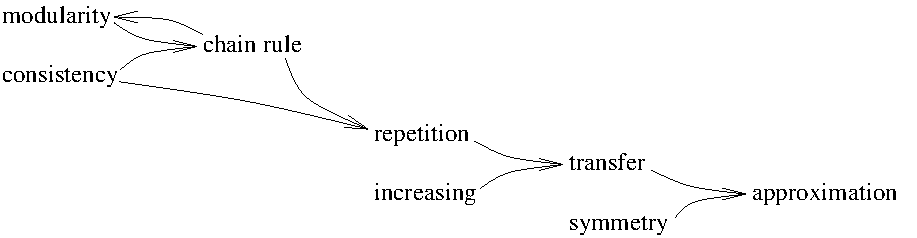
\includegraphics[width=122\unitlength]{mean_condns}}
\cell{25}{35}{c}{\scriptsize trivial}
\cell{15}{29.5}{c}{\scriptsize\ref{lemma:cons-mod-chn}}
\cell{35.5}{24}{c}{\scriptsize\ref{lemma:cons-chn-rep}}
\cell{64}{14}{c}{\scriptsize\ref{lemma:transfer}}
\cell{88}{9.7}{c}{\scriptsize\ref{lemma:approx}}
\end{picture}
\caption{Implications between properties of weighted means (Lemmas
  \ref{lemma:cons-mod-chn}--\ref{lemma:approx}).  The labels on the arrows
  indicate lemma numbers.}  
\lbl{fig:mean-condns}
\end{figure}
% 
The elementary implications (Lemmas
\ref{lemma:cons-mod-chn}--\ref{lemma:approx}) are shown in
Figure~\ref{fig:mean-condns}. In these lemmas, $I$ denotes a real interval
and $M$ denotes a sequence of functions $(M \from \Delta_n \times I^n \to
I)_{n \geq 1}$.  The properties of means mentioned there were all defined in
Section~\ref{sec:pwr-mns} (apart from transfer and approximation, defined
below) and are summarized in Appendix~\ref{app:condns}.

Plainly the chain rule implies modularity.  There is also a kind of
converse:

\begin{lemma}
\lbl{lemma:cons-mod-chn}
If $M$ is consistent and modular then $M$ satisfies the chain rule.
\end{lemma}

\begin{proof}
Let $\vc{w} \in \Delta_n$, let $\p^1 \in \Delta_{k_1}, \ldots, \p^n \in
\Delta_{k_n}$, and let $\vc{x}^1 \in I^{k_1}, \ldots, \vc{x}^n \in
I^{k_n}$, where $n, k_i \geq 1$ are integers.  Write $a_i = M(\p^i,
\vc{x}^i)$.  By consistency,
\[
M(\p^i, \vc{x}^i) = a_i = M\bigl(\vc{u}_1, (a_i)\bigr) 
\]
for each $i$.  Hence by modularity,
\[
M\bigl( 
\vc{w} \of (\p^1, \ldots, \p^n), 
\vc{x}^1 \oplus\cdots\oplus \vc{x}^n
\bigr)
=
M\bigl(
\vc{w} \of (\vc{u}_1, \ldots, \vc{u}_1),
(a^1) \oplus\cdots\oplus (a^n)
\bigr).
\]
But the right-hand side is $M\bigl(\vc{w}, (a_1, \ldots, a_n)\bigr)$, so
the result is proved.
\end{proof}

\begin{lemma}
\lbl{lemma:cons-chn-rep}
If $M$ is consistent and satisfies the chain rule then $M$ has the
repetition property.   
\end{lemma}

\begin{proof}
Let $\p \in \Delta_n$ and $\vc{x} \in I^n$; suppose that $x_i =
x_{i + 1}$ for some $i < n$.  We must prove that
% 
\begin{align*}
M(\p, \vc{x}) &
=
M\bigl(
(p_1, \ldots, p_{i - 1}, p_i + p_{i + 1}, p_{i + 2}, \ldots, p_n),      \\
&
\hspace*{2.5em}
% \quad\quad\,\,\,
(x_1, \ldots, x_{i - 1}, x_i, x_{i + 2}, \ldots, x_n)
\bigr).
\end{align*}
% 
For ease of notation, let us assume that $i = n - 1$.  (The general case is
similar.)  By Lemma~\ref{lemma:decomp},
\[
\p = 
(p_1, \ldots, p_{n - 2}, p_{n - 1} + p_n) \of
(\vc{u}_1, \ldots, \vc{u}_1, \vc{r})
\]
for some $\vc{r} \in \Delta_2$.  Then 
% 
\begin{align*}
M(\p, \vc{x})
&
=
M \bigl(
(p_1, \ldots, p_{n - 2}, p_{n - 1} + p_n) \of
(\vc{u}_1, \ldots, \vc{u}_1, \vc{r}),   \\
&
\hspace*{2.5em}
(x_1) \oplus\cdots\oplus (x_{n - 2}) \oplus (x_{n - 1}, x_{n - 1})
\bigr),
\end{align*}
% 
so by the chain rule and consistency,
% 
\begin{align*}
M(\p, \vc{x})   &
=
M \Bigl(
(p_1, \ldots, p_{n - 2}, p_{n - 1} + p_n),      \\
&
\hspace*{2.5em}
\bigl( 
M(\vc{u}_1, (x_1)), \ldots, M(\vc{u}_1, (x_{n - 2})), 
M(\vc{r}, (x_{n - 1}, x_{n - 1}))
\bigr)
\Bigr)  \\
&
=
M \bigl(
(p_1, \ldots, p_{n - 2}, p_{n - 1} + p_n),
(x_1, \ldots, x_{n - 2}, x_{n - 1})
\bigr),
\end{align*}
% 
as required.
\end{proof}

\begin{lemma}
\lbl{lemma:transfer}
If $M$ has the repetition property and is increasing, then $M$ also has the
\demph{transfer}%
%
\index{transfer property} 
% 
property:
\[
M(\p, \vc{x})
\leq
M \bigl( 
(p_1, \ldots, p_{i - 1}, 
p_i - \delta, p_{i + 1} + \delta, 
p_{i + 2}, \ldots, p_n),
\vc{x}
\bigr)
\]
whenever $1 \leq i < n$, $\p \in \Delta_n$, $\vc{x} \in I^n$ with $x_i
  \leq x_{i + 1}$, and $0 \leq \delta \leq p_i$.
\end{lemma}

The transfer property states that a weighted mean increases when
weight is transferred from a smaller argument to a larger one.

\begin{proof}
As in the last proof, we may harmlessly assume that $i = n - 1$.  We have
% 
\begin{align}
M(\p, \vc{x})   &
=
M\bigl(
(p_1, \ldots, p_{n - 2}, p_{n - 1} - \delta, \delta, p_n),
(x_1, \ldots, x_{n - 2}, x_{n - 1}, x_{n - 1}, x_n)
\bigr)  
\lbl{eq:trans-1}      \\
&
\leq
M\bigl(
(p_1, \ldots, p_{n - 2}, p_{n - 1} - \delta, \delta, p_n),
(x_1, \ldots, x_{n - 2}, x_{n - 1}, x_n, x_n)
\bigr)  
\lbl{eq:trans-2}      \\
&
=
M\bigl(
(p_1, \ldots, p_{n - 2}, p_{n - 1} - \delta, p_n + \delta),
\vc{x}
\bigr),
\lbl{eq:trans-3}
\end{align}
% 
where~\eqref{eq:trans-1} and~\eqref{eq:trans-3} hold by repetition
and~\eqref{eq:trans-2} holds because $M$ is increasing.
\end{proof}

\begin{lemma}
\lbl{lemma:approx}
Suppose that $M$ is symmetric and has the transfer property.  Then $M$ also
has the following \demph{approximation}%
%
\index{approximation property}
% 
property: for all $\p \in \Delta_n$, $\vc{x} \in I^n$ and $\delta > 0$,
there exist $\p^-, \p^+ \in \Delta_n$ such that all the coordinates of
$\p^-$ and $\p^+$ are rational,
\[
\max_i |p^-_i - p_i| < \delta,
\quad
\max_i |p^+_i - p_i| < \delta,
\]
and
\[
M(\p^-, \vc{x}) \leq M(\p, \vc{x}) \leq M(\p^+, \vc{x}).
\]
\end{lemma}

\begin{proof}
We just prove the existence of such a $\p^+$, the argument for $\p^-$ being
similar.  By symmetry, we may assume that $x_1 \leq \cdots \leq x_n$.

Choose $\delta_1 \in [0, \delta)$ with $0 \leq p_1 - \delta \in \Q$.  By
  the transfer property,
\[
M(\p, \vc{x})
\leq
M\bigl(
(p_1 - \delta_1, p_2 + \delta_1, p_3, \ldots, p_n), 
\vc{x}
\bigr).
\]
Next, choose $\delta_2 \in [0, \delta)$ such that $0 \leq p_2 + \delta_1 -
  \delta_2 \in \Q$.  By the transfer property,
% 
\begin{multline*}
M\bigl(
(p_1 - \delta_1, p_2 + \delta_1, p_3, \ldots, p_n), 
\vc{x}
\bigr)
\\
\leq
M\bigl(
(p_1 - \delta_1, p_2 + \delta_1 - \delta_2, p_3 + \delta_2, p_4, 
\ldots, p_n), 
\vc{x}
\bigr).
\end{multline*}
% 
Continuing in this way, we obtain $n - 1$ inequalities that together imply
that 
\[
M(\p, \vc{x})
\leq
M\bigl(
(p_1 - \delta_1, 
p_2 + \delta_1 - \delta_2, \ldots, 
p_{n - 1} + \delta_{n - 2} - \delta_{n - 1}, 
p_n + \delta_{n - 1}),
\vc{x}
\bigr).
\]
The result follows by taking $\p^+$ to be the distribution on the
right-hand side. 
\end{proof}

Many properties of weighted means $M(-, -)$ imply the corresponding
property of their unweighted counterparts $M(\vc{u}_n, -)$:

\begin{lemma}
Let $I$ be an interval and let $(M \from \Delta_n \times I^n \to I)_{n
  \geq 1}$ be a sequence of functions.  If $M$ is symmetric, consistent,
increasing, or strictly increasing (respectively), then so is the sequence of
functions $\bigl(M(\vc{u}_n, -) \from I^n \to I\bigr)_{n \geq 1}$.
Moreover, if $I$ is closed under multiplication and $M$ is homogeneous then
so is $(M(\vc{u}_n, -))_{n \geq 1}$.  
\end{lemma}

\begin{proof}
Trivial.
\end{proof}

It was stated on p.~\pageref{p:decomp-analogue} that decomposability is
an unweighted analogue of the chain rule.  The following lemma supports
that claim.

\begin{lemma}
\lbl{lemma:u-w-decomp}
Let $I$ be a real interval and let $(M \from \Delta_n \times I^n \to I)_{n
  \geq 1}$ be a sequence of functions that is consistent and satisfies the
chain rule.  Then $\bigl( M(\vc{u}_n, -)\from I^n \to I\bigr)_{n \geq 1}$
is decomposable.
\end{lemma}

\begin{proof}
Let $n, k_1, \ldots, k_n \geq 1$ and $\vc{x}^1 \in I^{k_1}, \ldots,
\vc{x}^n \in I^{k_n}$.  Write $a_i = M(\vc{u}_{k_i}, \vc{x}^i)$ and $k =
\sum k_i$.  We must show that
\[
M(\vc{u}_k, \vc{x}^1 \oplus\cdots\oplus \vc{x}^n)
=
M\bigl(\vc{u}_k, (k_1 \mc a_1, \ldots, k_n \mc a_n)\bigr).
\]
We have
\[
\vc{u}_k
=
(k_1/k, \ldots, k_n/k) \of (\vc{u}_{k_1}, \ldots, \vc{u}_{k_n}),
\]
so by the chain rule,
% 
\begin{equation}
\lbl{eq:uwd-1}
M(\vc{u}_k, \vc{x}^1 \oplus\cdots\oplus \vc{x}^n)
=
M\bigl(
(k_1/k, \ldots, k_n/k), (a_1, \ldots, a_n)
\bigr).
\end{equation}
% 
But by Lemma~\ref{lemma:cons-chn-rep}, $M$ has the repetition property,
which implies by induction that the right-hand side of~\eqref{eq:uwd-1} is
equal to 
\[
M\bigl(\vc{u}_k, (k_1 \mc a_1, \ldots, k_n \mc a_n)\bigr).
\]
This completes the proof.
\end{proof}

We now make a tool for converting theorems on unweighted means into
theorems on weighted means.

\begin{propn}
\lbl{propn:u-to-w}
\index{mean!weighted vs.\ unweighted}
% 
Let $I$ be a real interval and let 
\[
\bigl( M, M' \from \Delta_n \times I^n \to I \bigr)_{n \geq 1}
\]
be two sequences of functions.  Suppose that:
% 
\begin{enumerate}
\item 
both $M$ and $M'$ have the absence-invariance and repetition properties;

\item
$M$ is symmetric and increasing;

\item
for each $\vc{x} \in I^n$, the function $M'(-, \vc{x})$ is continuous on
the open simplex $\Delta_n^\circ$.
\end{enumerate}
% 
Suppose also that
\[
M(\vc{u}_n, -) = M'(\vc{u}_n, -) \from I^n \to I
\]
for all $n \geq 1$.  Then $M = M'$.
\end{propn}

\begin{proof}
First we prove that $M(\p, -) = M'(\p, -)$ when the coordinates of $\p$ are
rational and nonzero.  Write
\[
\p = (k_1/k, \ldots, k_n/k),
\]
where $k_1, \ldots, k_n$ are positive integers and $k = \sum k_i$.  Let
$\vc{x} \in I^n$.  Then by the repetition property of $M$ and induction,
% 
\begin{equation}
\lbl{eq:utw-1}
M(\p, \vc{x})
=
M\bigl( \vc{u}_k,
(k_1 \mc x_1, \ldots, k_n \mc x_n)
\bigr).
\end{equation}
% 
The same argument applied to $M'$ gives
% 
\begin{equation}
\lbl{eq:utw-2}
M'(\p, \vc{x})
=
M'\bigl( \vc{u}_k,
(k_1 \mc x_1, \ldots, k_n \mc x_n)
\bigr).
\end{equation}
% 
But the right-hand sides of~\eqref{eq:utw-1} and~\eqref{eq:utw-2} are
equal by hypothesis, so $M(\p, \vc{x}) = M'(\p, \vc{x})$.

Now we show by induction on $n \geq 1$ that $M(\p, \vc{x}) = M'(\p,
\vc{x})$ for all $\p \in \Delta_n$ and $\vc{x} \in I^n$.  

For $n = 1$, we must have $\p = \vc{u}_1$, hence $M(\p, \vc{x}) = M'(\p,
\vc{x})$ by hypothesis.

Let $n \geq 2$ and assume the result for $n - 1$.  If $p_i =
0$ for some $i$ then $M(\p, \vc{x}) = M'(\p, \vc{x})$ by inductive
hypothesis and absence-invariance of $M$ and $M'$.  Suppose, then,
that $\p \in \Delta_n^\circ$.

Let $\epsln > 0$.  Since $M'(-, \vc{x})$ is continuous at $\p$, we can
choose $\delta \in (0, \min_i p_i)$ such that for $\vc{r} \in
\Delta_n^\circ$,
\[
\max_i |p_i - r_i| < \delta
\implies
|M'(\p, \vc{x}) - M'(\vc{r}, \vc{x})| < \epsln.
\]
By Lemma~\ref{lemma:transfer}, $M$ has the transfer property, so by
Lemma~\ref{lemma:approx}, $M$ also has the approximation property.  Choose
$\p^+$ as in Lemma~\ref{lemma:approx}; then
% 
\begin{equation}
\lbl{eq:utw-3}
|M'(\p, \vc{x}) - M'(\p^+, \vc{x})| < \epsln.
\end{equation}
% 
Also, since $\p \in \Delta_n^\circ$ and 
\[
\max_i |p_i - p^+_i| < \delta < \min_i p_i,
\]
we have $\p^+ \in \Delta_n^\circ$ too.  Now
% 
\begin{align}
M(\p, \vc{x})   &
\leq
M(\p^+, \vc{x}) 
\lbl{eq:utw-4}        \\
&
=
M'(\p^+, \vc{x})
\lbl{eq:utw-5}        \\
&
<
M'(\p, \vc{x}) + \epsln,
\lbl{eq:utw-6}
\end{align}
% 
where inequality~\eqref{eq:utw-4} is one of the defining properties of
$\p^+$, equation~\eqref{eq:utw-5} holds because the coordinates of $\p^+$
are rational and nonzero (using the first step of the proof), and
inequality~\eqref{eq:utw-6} follows from~\eqref{eq:utw-3}.  But
this holds for all $\epsln > 0$, so
\[
M(\p, \vc{x}) \leq M'(\p, \vc{x}).
\]
A very similar argument, using the distribution $\p^-$ of
Lemma~\ref{lemma:approx}, proves the opposite inequality.  Hence $M(\p,
\vc{x}) = M'(\p, \vc{x})$, completing the proof.
\end{proof}

We can now simply read off four characterization theorems for weighted
power means.  They are summarized in Table~\ref{table:w-mn-thms}, and are
derived from the four theorems on unweighted means shown in
Table~\ref{table:mn-thms}.

\begin{thm}
\lbl{thm:w-str-inc}
\index{power mean!characterization of!weighted on $(0, \infty)$}
% 
Let $\bigl( M \from \Delta_n \times (0, \infty)^n \to (0, \infty) \bigr)_{n
  \geq 1}$ be a sequence of functions.  The following are equivalent:
% 
\begin{enumerate}
\item 
\lbl{part:w-str-inc-condns}
$M$ is symmetric, absence-invariant, consistent, strictly increasing,
modular, and homogeneous;

\item
\lbl{part:w-str-inc-form}
$M = M_t$ for some $t \in (-\infty, \infty)$.
\end{enumerate}
\end{thm}

\begin{proof}
Part~\bref{part:w-str-inc-form} implies part~\bref{part:w-str-inc-condns}
by the results in Section~\ref{sec:pwr-mns}.
Now assume~\bref{part:w-str-inc-condns}.
The unweighted mean
\[
\bigl( 
M(\vc{u}_n, -) \from (0, \infty)^n \to (0, \infty)
\bigr)_{n \geq 1}
\]
is symmetric, strictly increasing, decomposable, and homogeneous (using
Lemmas~\ref{lemma:cons-mod-chn} and~\ref{lemma:u-w-decomp} for
decomposability).  Hence by Theorem~\ref{thm:str-inc}, there is some $t \in
(-\infty, \infty)$ such that
\[
M(\vc{u}_n, -) = M_t(\vc{u}_n, -)
\]
for all $n \geq 1$.  By Lemmas~\ref{lemma:cons-mod-chn}
and~\ref{lemma:cons-chn-rep}, $M$ has the repetition property.  Hence by the
previously-established properties of $M_t$, we can apply
Proposition~\ref{propn:u-to-w} with $M' = M_t$, giving $M = M_t$.
\end{proof}

Theorem~\ref{thm:w-str-inc} is essentially due to Hardy,%
%
\index{Hardy, Godfrey Harold} 
%
Littlewood%
%
\index{Littlewood, John Edensor}
%
and P\'olya~\cite{HLP}.%
%
\index{Polya, George@P\'olya, George}
% 
Some minor details aside, it is the conjunction of
their Theorems~84 and~215, translated out of the language of Stieltjes
integrals and into elementary terms.  Section~6.21 of~\cite{HLP} gives
details.

\begin{thm}
\lbl{thm:w-zero-str-inc}
\index{power mean!characterization of!weighted on $[0, \infty)$}
% 
Let $\bigl( M \from \Delta_n \times [0, \infty)^n \to [0, \infty) \bigr)_{n
  \geq 1}$ be a sequence of functions.  The following are equivalent:
% 
\begin{enumerate}
\item 
$M$ is symmetric, absence-invariant, consistent, strictly increasing,
  modular, and homogeneous;

\item
$M = M_t$ for some $t \in (0, \infty)$.
\end{enumerate}
\end{thm}

\begin{proof}
This follows by exactly the same argument as for the last theorem, but
using Theorem~\ref{thm:zero-str-inc} instead of Theorem~\ref{thm:str-inc}.
\end{proof}


\begin{thm}
\lbl{thm:w-inc}
\index{power mean!characterization of!weighted on $(0, \infty)$}
% 
Let $\bigl( M \from \Delta_n \times (0, \infty)^n \to (0, \infty) \bigr)_{n
  \geq 1}$ be a sequence of functions.  The following are equivalent:
% 
\begin{enumerate}
\item 
$M$ is symmetric, absence-invariant, consistent, increasing, modular, and
  homogeneous;

\item
$M = M_t$ for some $t \in [-\infty, \infty]$.
\end{enumerate}
\end{thm}

\begin{proof}
This follows from Theorem~\ref{thm:inc} by the same argument.
\end{proof}


\begin{thm}
\lbl{thm:w-cts-inc}
\index{power mean!characterization of!weighted on $[0, \infty)$}
% 
Let $\bigl( M \from \Delta_n \times [0, \infty)^n \to [0, \infty) \bigr)_{n
  \geq 1}$ be a sequence of functions.  The following are equivalent:
% 
\begin{enumerate}
\item 
$M$ is symmetric, absence-invariant, consistent, increasing, modular,
  homogeneous, and continuous in its second argument;

\item
$M = M_t$ for some $t \in [-\infty, \infty]$.
\end{enumerate}
\end{thm}

\begin{proof}
This follows from Theorem~\ref{thm:cts-inc} by the same argument again,
this time also noting that by consistency, none of the functions
$M(\vc{u}_n, -)$ is identically zero.  
\end{proof}

We will use Theorem~\ref{thm:w-inc} to prove an axiomatic characterization
of measures of the value of a community (Section~\ref{sec:value-char}) and,
building on this, to characterize the Hill numbers
(Section~\ref{sec:total-hill}).




